\documentclass[11pt]{article}

% ----- Packages -----
\usepackage[a4paper,margin=1in]{geometry}
\usepackage{times}
\usepackage{microtype}
\usepackage{graphicx}
\usepackage{grffile}
% Search figures relative to this tex file
\graphicspath{{./figs/}}
% Prefer vector graphics when available
\DeclareGraphicsExtensions{.pdf,.png,.jpg}
\usepackage{booktabs}
\usepackage{amsmath,amsfonts,amssymb,amsthm}
\usepackage{mathtools}
\usepackage{multirow}
\usepackage{enumitem}
\usepackage{caption}
\usepackage{subcaption}
\usepackage{xcolor}
\usepackage{hyperref}
\usepackage[skins,most]{tcolorbox}
\hypersetup{colorlinks=true, allcolors=blue!70!black}
\usepackage[numbers]{natbib}

% TikZ for conceptual schematic
\usepackage{tikz}
\usetikzlibrary{arrows.meta,positioning,shapes.geometric,calc}

% ----- Theorem-like environments -----
\newtheorem{proposition}{Proposition}
\newtheorem{definition}{Definition}

% ----- Macros -----
\newcommand{\RR}{\mathbb{R}}
\newcommand{\1}{\mathbf{1}}
\newcommand{\diag}{\mathrm{diag}}
\newcommand{\tr}{\mathrm{tr}}
\newcommand{\E}{\mathbb{E}}
\newcommand{\Var}{\mathrm{Var}}
\newcommand{\PSD}{\succeq 0}
\newcommand{\NSD}{\preceq 0}
\newcommand{\ip}[2]{\left\langle #1,\,#2\right\rangle}
% Ensure consistent negative-number rendering in text/tables
\newcommand{\negnum}[1]{\ensuremath{-#1}}

% ----- Title -----
\title{GeoCert: Coordinate-Free Geometric Consistency Tests\\
for LLM Representations}

\author{Elijah Lucas\\
\tiny contact: elijah.lucas.research@gmail.com}

\date{}

\begin{document}
\maketitle

\begin{abstract}
\textbf{Simple summary.} We test a basic question about model representations: do all the pairwise relationships between hidden states fit inside a single, ordinary geometric space? If yes, common tools (neighbors, clustering, PCA/MDS) are trustworthy; if not, they can silently distort. \textbf{Method in one line.} We map similarities to distances, check a convex feasibility condition from distance geometry, and use the bottom eigenvalue as a global ``consistency meter.'' We then explain failures by splitting edges into two minimal layers.
\end{abstract}

\vspace{-0.5em}
\section{Introduction}
Pairwise similarities underlie core tools in representation analysis (nearest neighbors, clustering, linear probes, MDS/PCA). These methods implicitly assume a \emph{single Euclidean chart}. We study the validity of this assumption in large language models (LLMs). Our central question: \textbf{do observed pairwise relations admit a single Euclidean embedding?} If not, \emph{where} and \emph{why} do they fail?

\paragraph{Intuition (what and why).} Geometric inconsistency means the pairwise relationships written by different contexts cannot be explained within one global Euclidean geometry at once. Practically, this signals that the model is stitching together incompatible relational programs across contexts: the same pair can be near in one setting and far in another in a way that no single embedding can satisfy. We care because this reveals where models may be brittle, modular, or conflict-driven---and because a simple, global certificate lets us diagnose such clashes without coordinates, parameters, or specific probes.

A single Euclidean chart is the quiet assumption behind nearest-neighbor retrieval, clustering, and linear projections. When relations come from heterogeneous contexts, that assumption can fail globally even if most local triangles look fine. Consider measuring distances between 4 cities and finding: A--B = 100 miles, B--C = 100 miles, C--D = 100 miles, but A--D = 50 miles. No matter how you arrange these cities on a map, something's wrong---these distances can't all be true simultaneously. GeoCert catches these impossible distance relationships in representation space, provides a coordinate-free test of geometric consistency, pinpoints the edges/nodes that contradict it, and shows that a simple two-layer split resolves nearly all contradictions across three model families.

% ===================== Conceptual Figure (FIXED) =====================
\begin{figure}[t]
\centering
\begin{subfigure}[t]{0.32\textwidth}
\centering
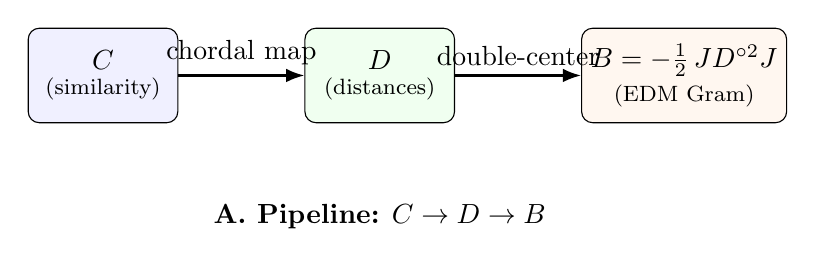
\begin{tikzpicture}[>=Latex, node distance=1.6cm]
\node[draw,rounded corners,minimum width=1.9cm,minimum height=1.2cm,fill=blue!6] (C)
  {\shortstack{$C$\\\footnotesize (similarity)}};
\node[draw,rounded corners,minimum width=1.9cm,minimum height=1.2cm,fill=green!6,right=of C] (D)
  {\shortstack{$D$\\\footnotesize (distances)}};
\node[draw,rounded corners,minimum width=2.2cm,minimum height=1.2cm,fill=orange!6,right=of D] (B)
  {\shortstack{$B=-\tfrac12\,J D^{\circ2} J$\\\footnotesize (EDM Gram)}};
\draw[->,thick] (C) -- node[above]{chordal map} (D);
\draw[->,thick] (D) -- node[above]{double-center} (B);
\node[below=0.9cm of D,align=center] {\textbf{A. Pipeline:} $C \to D \to B$};
\end{tikzpicture}
\end{subfigure}\hfill
\begin{subfigure}[t]{0.32\textwidth}
\centering
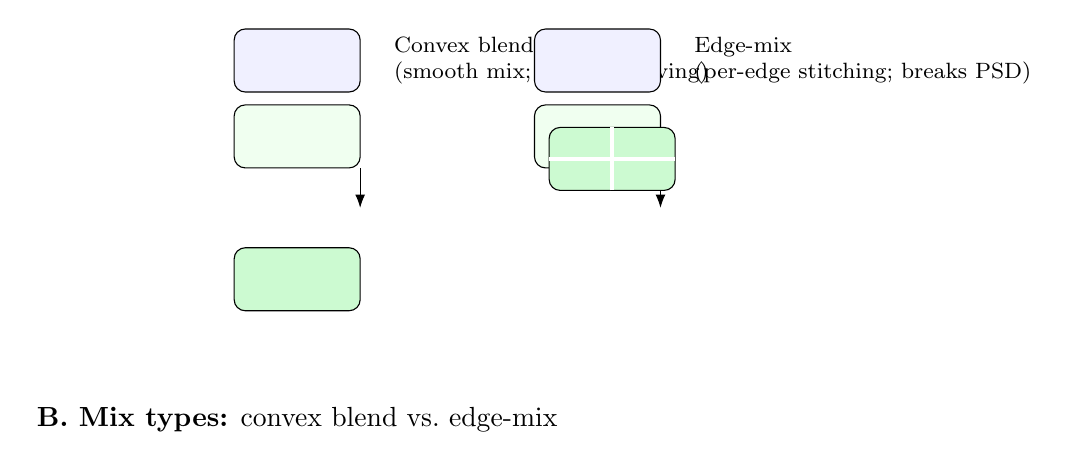
\begin{tikzpicture}[>=Latex]
% Convex blend
\node[draw,rounded corners,fill=blue!6,minimum width=1.6cm,minimum height=0.8cm] (c1) {};
\node[draw,rounded corners,fill=green!6,minimum width=1.6cm,minimum height=0.8cm,below=0.15cm of c1] (c2) {};
\node[right=0.3cm of c1,align=left,font=\footnotesize] {Convex blend\\(smooth mix; PSD-preserving)};
\draw[->] ([xshift=0.8cm]c2.south) -- ++(0,-0.5cm);
\node[draw,rounded corners,fill=blue!10!green!20,minimum width=1.6cm,minimum height=0.8cm,below=1.0cm of c2] (cb) {};
% Edge mix
\node[draw,rounded corners,fill=blue!6,minimum width=1.6cm,minimum height=0.8cm,right=2.2cm of c1] (e1) {};
\node[draw,rounded corners,fill=green!6,minimum width=1.6cm,minimum height=0.8cm,below=0.15cm of e1] (e2) {};
\node[right=0.3cm of e1,align=left,font=\footnotesize] {Edge-mix\\(per-edge stitching; breaks PSD)};
\draw[->] ([xshift=0.8cm]e2.south) -- ++(0,-0.5cm);
\begin{scope}[shift={(3.2cm,-1.65cm)}]
  \draw[rounded corners,fill=blue!10!green!20] (0,0) rectangle (1.6,0.8);
  \draw[very thick,white] (0.0,0.4) -- (1.6,0.4);
  \draw[very thick,white] (0.8,0.0) -- (0.8,0.8);
\end{scope}
\node[below=1.1cm of cb,align=center] {\textbf{B. Mix types:} convex blend vs.\ edge-mix};
\end{tikzpicture}
\end{subfigure}\hfill
\begin{subfigure}[t]{0.32\textwidth}
\centering
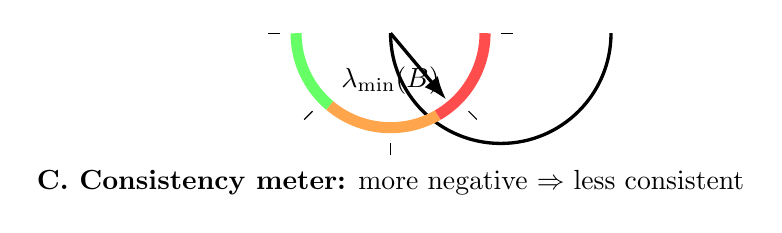
\begin{tikzpicture}[>=Latex]
% Gauge
\draw[very thick] (0,0) arc[start angle=180,end angle=360,radius=1.4];
\foreach \a in {180,225,270,315,360}{
  \draw[thin] ({1.4*cos(\a)},{1.4*sin(\a)}) -- ({1.55*cos(\a)},{1.55*sin(\a)});
}
% colored ticks (conceptual)
\draw[line width=4pt,green!60] (180:1.2) arc (180:230:1.2);
\draw[line width=4pt,orange!70] (230:1.2) arc (230:300:1.2);
\draw[line width=4pt,red!70] (300:1.2) arc (300:360:1.2);
% needle
\draw[very thick,->] (0,0) -- ({1.1*cos(310)},{1.1*sin(310)});
\node[below=2ex] at (0,0) {$\lambda_{\min}(B)$};
\node at (0,-1.9) {\textbf{C. Consistency meter:} more negative $\Rightarrow$ less consistent};
\end{tikzpicture}
\end{subfigure}
\caption{\textbf{Conceptual schematic.} \textbf{A:} GeoCert pipeline from similarities $C$ to distances $D$ to the EDM Gram $B$. \textbf{B:} \emph{Convex blends} preserve PSD (smooth mix), whereas \emph{edge-mixes} stitch per-edge constraints and can break PSD. \textbf{C:} The bottom eigenvalue $\lambda_{\min}(B)$ serves as a global ``consistency meter.'' \textbf{What to notice:} GeoCert is coordinate-free, distinguishes safe blends from unsafe mixing, and quantifies global inconsistency with a single spectrum witness.}
\label{fig:concept}
\end{figure}
% ======================================================================

\begin{tcolorbox}[colback=gray!5!white,colframe=gray!75!black,title=How to read GeoCert]
\textbf{1. Question.} Do mixed-context representations fit one consistent Euclidean geometry?\\
\textbf{2. Test.} Map similarities $\to$ distances, form $B$; $\lambda_{\min}(B){<}0$ certifies global inconsistency.\\
\textbf{3. Controls.} Convex blends are PSD-preserving and stay near $0$; edge-mix produces U-dips.\\
\textbf{4. Diagnosis.} Edge tension $\tau$ and node load $L$ localize bridges under stress.\\
\textbf{5. Fix.} A minimal $K{=}2$ split removes $\sim$95--97\% of negative mass on residuals; heads project to exact PSD per layer.
\end{tcolorbox}

\noindent\textbf{GeoCert}, a coordinate-free pipeline that maps similarities $C$ to Euclidean distances $D$, forms the EDM Gram $B=-\tfrac12\,J D^{\circ2} J$, and uses the bottom spectrum (e.g., $\lambda_{\min}(B)$ and negative-PSD mass) as \emph{global witnesses} of embeddability. We formally distinguish \emph{convex blends} of contexts (PSD-preserving; pass) from \emph{edge-mixes} (per-edge selection; break PSD; fail), explaining the characteristic U-curves we observe under edge-mix. We add local triangle scans, edge tension, node negative-load, and a greedy $K{=}2$ edge-level disentangling that explains failures by partitioning edges into two EDM-compatible layers (cf. \citep{schoenberg1938,gower1985,LibertiLavor2017,Dokmanic2015}).

\paragraph{Contributions.}
\begin{itemize}[leftmargin=1.5em]
\item \textbf{Global certificate.} EDM feasibility ($B \PSD$) yields noise-robust, coordinate-free PSD certificates and \emph{eigenvalue witnesses} ($\lambda_{\min}(B)\le 0$ with witness eigenvector).
\item \textbf{Mixture clarity.} We formalize \emph{convex blend} (PSD-preserving; pass) vs \emph{edge-mix} (per-edge selection; break PSD) and show U-curves arise from the latter.
\item \textbf{Explanations.} A greedy \textbf{$K{=}2$ edge assignment} removes \textbf{95--97\%} of negative mass on residual graphs; heads project to exact PSD.
\item \textbf{Breadth.} Results replicate across \textbf{OPT-125M}, \textbf{GPT-Neo-125M}, \textbf{DistilGPT2} (3 seeds), with bootstrap CIs and controls. \emph{GeoCert is a global, coordinate-free diagnostic that complements circuit-style local analyses.}
\end{itemize}

\section{Related Work}
\textbf{Metric/manifold learning.} Classical MDS assumes a single geometry; we \emph{test} this assumption with convex certificates \citep{torgerson1952,borg2005}.\\
\textbf{Inequality-based checks.} Local algebraic inequalities (triangle, hypermetric) are fragile under noise; GeoCert’s PSD tests are global.\\
\textbf{LLM interpretability.} Circuit/head analyses localize behaviors; we add a \emph{global compatibility} lens and a principled way to \emph{separate contextual layers} \citep{Vig2020CausalMediation,Elazar2021Amnesic,Meng2022ROME}.

\section{Methods}
\subsection{From similarities to EDMs}\label{sec:fromCtoB}
% ----- Glossary table updated to include plain English -----
\begin{table}[t]
\centering
\caption{Notation/glossary (core objects with plain-English meaning).}
\begin{tabular}{lll}
\toprule
Symbol & Definition & Plain meaning \\
\midrule
$C$ & Cosine similarity ($C\PSD$, $\diag(C)=\mathbf{1}$) & How much two states ``rhyme'' \\
$D$ & Chordal distances $D_{ij}=\sqrt{2(1-C_{ij})}$ & Turn similarity into distance \\
$J$ & Centering $I-\tfrac1n\,\mathbf{1}\mathbf{1}^\top$ & Remove average location \\
$B$ & EDM Gram $-\tfrac12\,J\,D^{\circ2}\,J$ & Global consistency check space \\
$\lambda_{\min}$ & Bottom eigenvalue of $B$ & Consistency meter (negative = fail) \\
Neg-mass & $\sum_{\lambda_k< -\varepsilon}|\lambda_k|$ & Size of global inconsistency \\
$\tau_{ij}$ & $(\hat u_i-\hat u_j)^2$ with $\hat u=Ju$ & Stress of edge $(i,j)$ \\
$L_i$ & $(B_-)_{ii}$ & Node's share of negative stress \\
\bottomrule
\end{tabular}
\end{table}

\paragraph{Notation.} We use $C$ for cosine similarity ($C\PSD$, $\diag(C)=\mathbf{1}$), $D$ for chordal distances $D_{ij}=\sqrt{2(1-C_{ij})}$, $J=I-\tfrac1n\,\mathbf{1}\mathbf{1}^\top$ for centering, and $B=-\tfrac12\,J\,D^{\circ2}\,J$ for the EDM Gram. Edge tension is $\tau_{ij}=(\hat u_i-\hat u_j)^2$ for worst eigenvector $u$ with $\hat u=Ju$, node negative-load is $L_i=(B_-)_{ii}$, and ``neg-mass'' is $\sum_{\lambda_k< -\varepsilon}|\lambda_k|$ with $\varepsilon\!\approx\!10^{-6}$.
For unit-normalized representations $(x_i)$ with cosine similarities $C_{ij}=\ip{x_i}{x_j}$, define \emph{chordal distances}
\[
d_{ij}=\sqrt{2(1-C_{ij})},\quad d_{ii}=0,
\]
and the centering matrix $J=I-\tfrac1n \1\1^\top$. The double-centered Gram of $D$ is
\[
B \;=\; -\tfrac12\, J\, D^{\circ2}\, J.\footnote{$D^{\circ2}$ denotes the elementwise square of distances (squared-chordal).}
\]

\begin{tcolorbox}[colback=blue!3,colframe=blue!40!black,title=Intuition (for \S\ref{sec:fromCtoB})]
\textbf{``How much do two states rhyme?''} $C$ says who is similar; $D$ turns that into distances; $B$ asks if all those distances can live on one ordinary map at once. If $B$ goes negative, the map tears.
\end{tcolorbox}

\begin{proposition}[Chordal mapping preserves EDM feasibility]
If $C \PSD$ with $\diag(C)=\1$, then $B= JCJ \PSD$, hence $D$ is an EDM.
\end{proposition}
\textit{Sketch.} Since $D^{\circ2}=2(1-C)$, we have $B=-J(I-C)J=JCJ$. For any $v$, $(Jv)^\top C (Jv)\ge 0$ as $C \PSD$ and $J$ is a projection. $\square$

\paragraph{Witnesses.} $\lambda_{\min}(B)\le 0$ certifies global inconsistency; the \emph{negative-PSD mass} $\sum_{\lambda_k<-\varepsilon}|\lambda_k|$ (we use $\varepsilon\!\approx\!10^{-6}$) is noise-robust.

\paragraph{Numerics (enforcement and dtype).} Before forming $D$ we enforce symmetry and unit diagonal: $C\leftarrow \tfrac12(C{+}C^\top)$ and $\diag(C){=}\mathbf{1}$; $D$ uses the chordal map with $\max(\cdot,0)$, and $B$ is symmetrized via $\tfrac12(B{+}B^\top)$. All linear algebra is run in \texttt{float64}.

\subsection{Edge-mix vs convex-blend}\label{sec:mix}
Given contexts $C^{(1)},C^{(2)}$ on the same nodes:
\begin{itemize}[leftmargin=1.5em]
\item \textbf{Convex blend:} $C^{(\rho)}=(1-\rho)C^{(1)}+\rho\,C^{(2)}$ preserves PSD $\Rightarrow$ chordal distances remain EDM-feasible; $\lambda_{\min}\approx 0$ across $\rho$.
\item \textbf{Edge-mix:} per-edge selection generally \emph{breaks Gram structure}, yielding $\lambda_{\min}\ll 0$ at mid-$\rho$ and pronounced U-curves.
\end{itemize}
This distinction mirrors practice: heterogeneous prompts/heads/layers write \emph{different} pairwise constraints, so naive edge mixing is the operational failure mode. We include \emph{convex-blend controls}.

\begin{tcolorbox}[colback=blue!3,colframe=blue!40!black,title=Intuition (for \S\ref{sec:mix})]
\textbf{``Stitching maps with different scales.''} Convex blends average maps smoothly. Edge-mix stitches edges from different maps---like taping two atlases with mismatched scales. The seams force a tear (negative eigenvalues).
\end{tcolorbox}

\subsection{Local vs global checks}\label{sec:localglobal}
\textbf{Triangles} (sampled triplets) catch local violations; \textbf{EDM PSD} aggregates \emph{all} constraints at once. We report both.

\begin{tcolorbox}[colback=blue!3,colframe=blue!40!black,title=Intuition (for \S\ref{sec:localglobal})]
\textbf{``Triangles are smoke; eigenvalues are the fire alarm.''} A few broken triangles may be noise (smoke). A strongly negative $\lambda_{\min}$ means the whole building violates geometry (fire).
\end{tcolorbox}

\subsection{Edge diagnostics and $K{=}2$ disentangling}\label{sec:k2}
Let $u$ be the worst eigenvector of $B$. With $\hat u=Ju$, define \textbf{edge tension}
\[
\tau_{ij} \;=\; (\hat u_i-\hat u_j)^2,
\]
and \textbf{node negative-load} from the negative spectral projector $B_-$, $L_i=(B_-)_{ii}=\sum_{\lambda_k<0}|\lambda_k|\,u_{k,i}^2$.
We rank top-$K$ edges by $\tau$ and alternatingly assign to two layers to \emph{minimize negative mass}. The procedure is monotone (local optimum). We use $K\!\approx\!2000$ for residual graphs and 5--7 alternations. For small head graphs, per-layer \emph{EDM projection} yields exact PSD.

\begin{tcolorbox}[colback=blue!3,colframe=blue!40!black,title=Intuition (for \S\ref{sec:k2})]
\textbf{``Two relational programs.''} The stress clusters along bridges between two compatible programs. Pulling them apart into $K{=}2$ layers relieves almost all tension.
\end{tcolorbox}

\subsection{Computational complexity \& scalability}
\textbf{Building $C$:} $O(n^2d)$; \textbf{forming $B$:} $O(n^2)$ time/memory; \textbf{eigen-witness:} bottom spectrum via Lanczos/power in $O(mn^2)$ ($m\!\ll\!n$). Triangles: $O(S)$ for $S$ samples. Disentangling: compute $\tau$ in $O(n^2)$ and alternate in $O(K)$ per iteration (5--7 iters).\\
\textbf{Scaling:} Nyström on $C$ (landmarks $p\!\ll\!n$), sparsified kNN subgraphs, randomized SVD/Lanczos \citep{halko2011}, and streaming rank-one updates with a few power iterations.

\subsection{Practical scaling via Nyström}\label{sec:nystrom}
For large $n$ we Nyström-approximate $C\approx W W^\top$ with $p\ll n$ landmarks \citep{williams2001nystrom,Fowlkes2004}, yielding $B\approx J W W^\top J$ and using Lanczos for bottom eigenpairs. This reduces memory to $O(np)$.

\section{Experimental Setup}
\textbf{Models:} \texttt{facebook/opt-125m}, \texttt{EleutherAI/gpt-neo-125M}, \texttt{distilgpt2}; scaling validation on \texttt{facebook/opt-350m} and \texttt{EleutherAI/pythia-1b} \citep{Zhang2022OPT,Biderman2023Pythia,Radford2019GPT2,Vaswani2017}.\\
\textbf{Features:} (i) \textbf{Residual} graphs at a mid layer; (ii) \textbf{Heads} graphs (66 edges) at a chosen layer.\\
\textbf{Sampling:} 3 seeds, 256 prompts, 21 $\rho$-steps; bootstrap CIs over seeds \citep{Efron1979}.\\
\textbf{Artifacts:} All figures under \texttt{figs/} and tables under \texttt{tables/}.\\[0.25em]
\textit{Layer choice.} We target a mid transformer block (L=8 for 125M/350M; L=5 for Distil) to avoid shallow features while capturing mixed computations in deeper layers. Results are qualitatively similar in adjacent layers.

\begin{tcolorbox}[title=Executive Summary]
\textbf{Question.} Do LLM representations from mixed contexts fit one consistent geometry? \\
\textbf{Test.} Map similarities to distances, form $B$; if $B$ has negative eigenvalues, the relations cannot be embedded in Euclidean space. \\
\textbf{Controls.} Convex blends (PSD-preserving) stay flat at $\lambda_{\min}\!\approx\!0$. \\
\textbf{Stress test.} Edge-mixing (per-edge from different contexts) yields U-curves with negative dips. \\
\textbf{Diagnosis.} Edge tension $\tau$ and node load $L$ locate the bridges under strain. \\
\textbf{Explanation.} A simple $K{=}2$ edge split removes 95--97\% of negative mass (residuals); head layers project to exact PSD. \\
\textbf{Relevance.} Stressed nodes predict causal importance (RFC alignment). \\
\textbf{Takeaway.} Models interleave a small number of compatible relational programs; GeoCert detects when a single chart is unsafe, shows where it fails, and how to separate it.
\end{tcolorbox}

% ===================== Main curves (now Fig. 2) =====================
\paragraph{Main curve figures.}
\begin{figure}[t]
\centering
\begin{subfigure}[t]{0.32\textwidth}
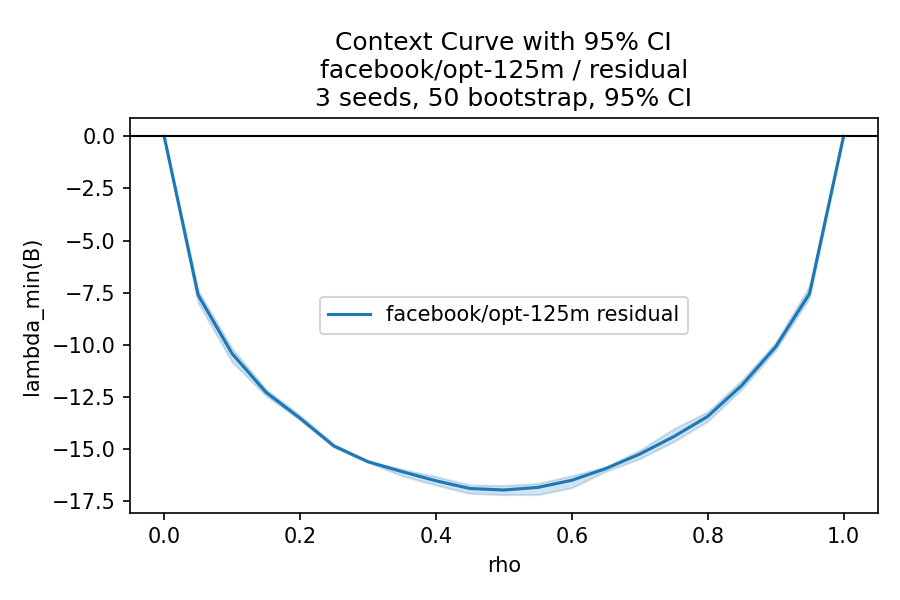
\includegraphics[width=\linewidth]{figs/curve_facebook_opt-125m_residual.png}
\caption{OPT residual}
\end{subfigure}\hfill
\begin{subfigure}[t]{0.32\textwidth}
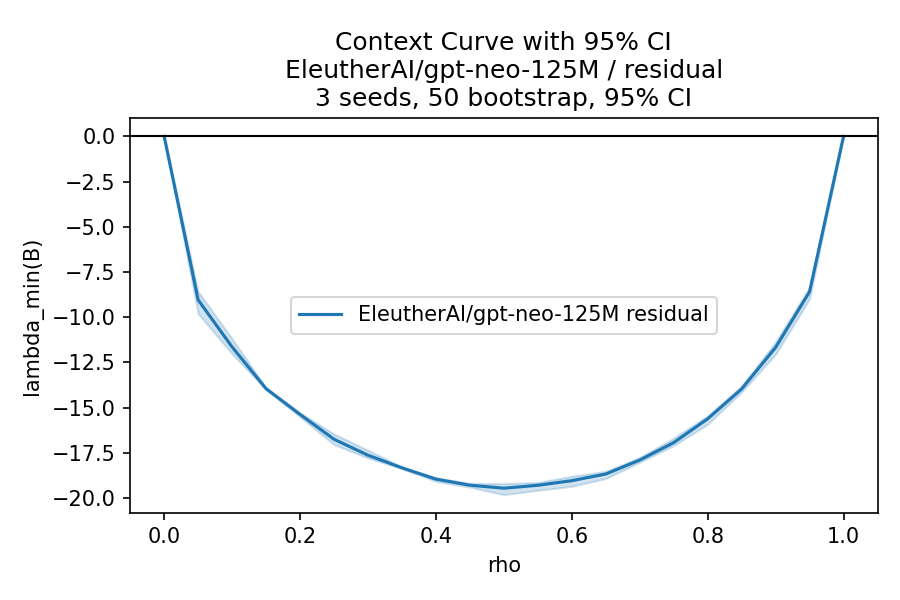
\includegraphics[width=\linewidth]{figs/curve_EleutherAI_gpt-neo-125M_residual.png}
\caption{GPT-Neo residual}
\end{subfigure}\hfill
\begin{subfigure}[t]{0.32\textwidth}
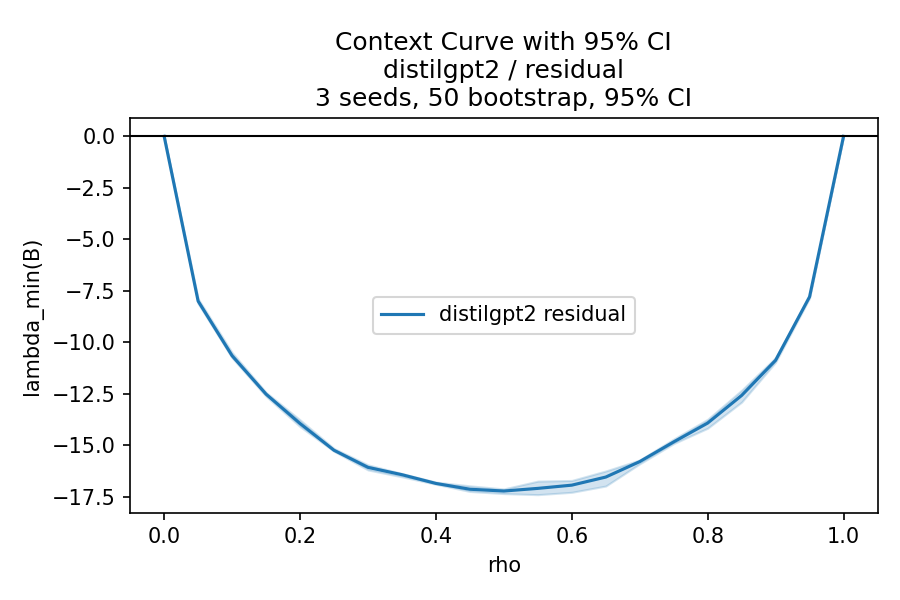
\includegraphics[width=\linewidth]{figs/curve_distilgpt2_residual.png}
\caption{Distil residual}
\end{subfigure}

\vspace{0.5em}

\begin{subfigure}[t]{0.32\textwidth}
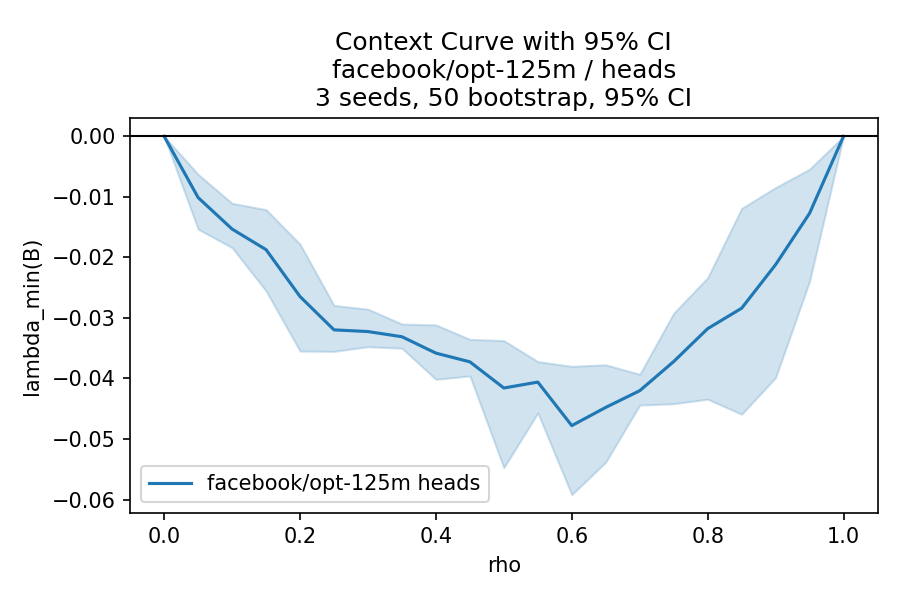
\includegraphics[width=\linewidth]{figs/curve_facebook_opt-125m_heads.png}
\caption{OPT heads}
\end{subfigure}\hfill
\begin{subfigure}[t]{0.32\textwidth}
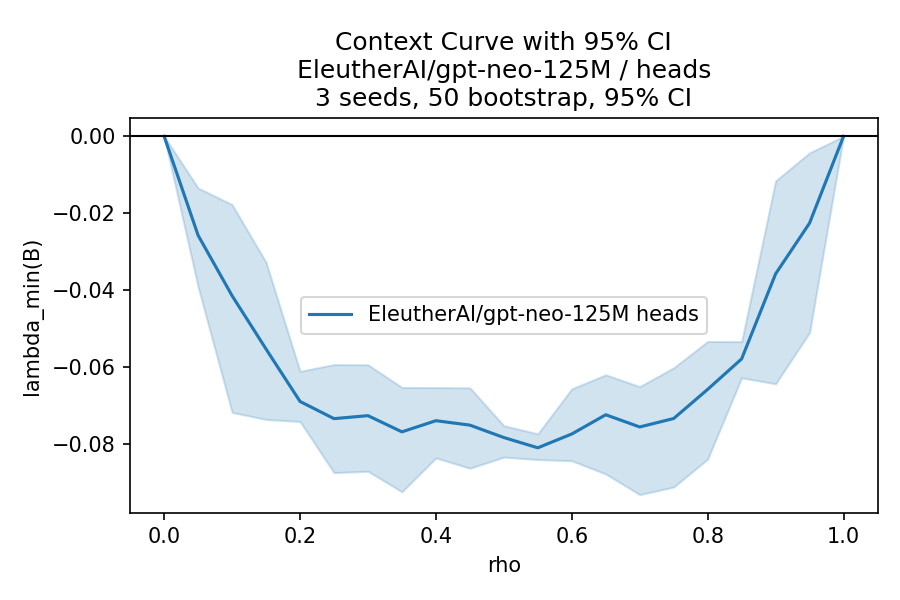
\includegraphics[width=\linewidth]{figs/curve_EleutherAI_gpt-neo-125M_heads.png}
\caption{GPT-Neo heads}
\end{subfigure}\hfill
\begin{subfigure}[t]{0.32\textwidth}
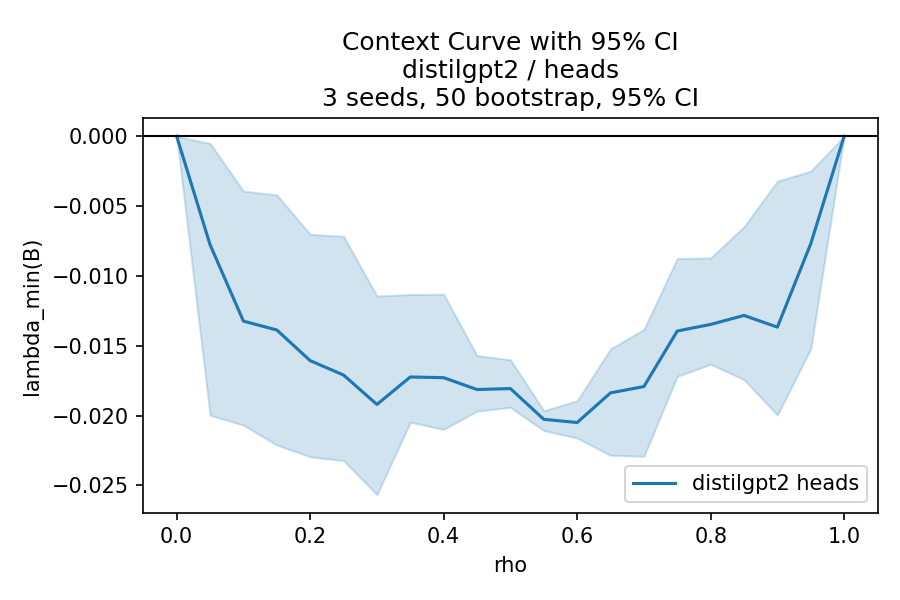
\includegraphics[width=\linewidth]{figs/curve_distilgpt2_heads.png}
\caption{Distil heads}
\end{subfigure}
\caption{Context-consistency curves ($\lambda_{\min}(B)$ vs $\rho$). \textbf{What to notice:} residual edge-mix produces pronounced U-curves with mid-$\rho$ dips (global inconsistency), while heads have small dips; convex-blend controls (not shown) remain flat near 0.}
\label{fig:curves}
\end{figure}

% ===================== Controls placed immediately after curves (Fig. 3) =====================
\begin{figure}[t]
\centering
\begin{subfigure}[t]{0.48\textwidth}
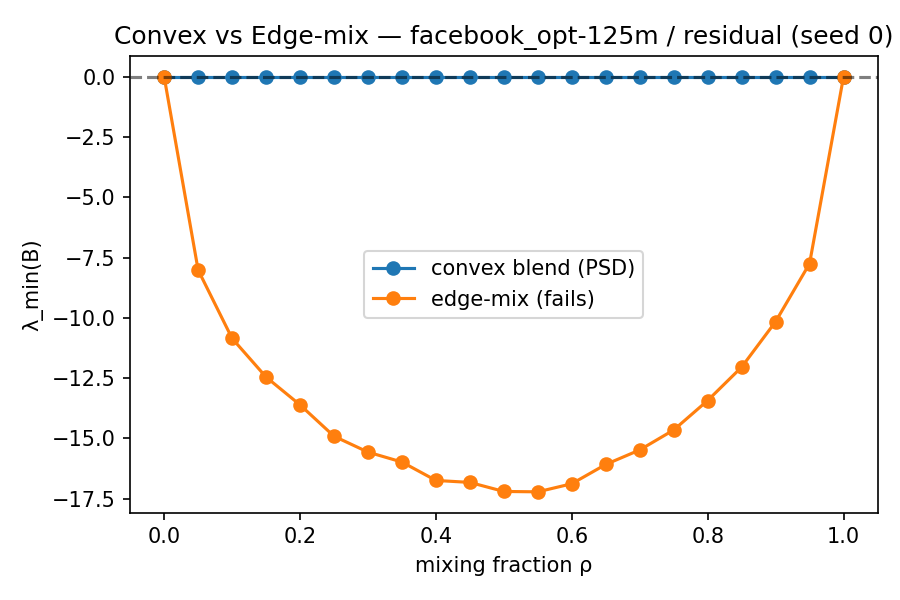
\includegraphics[width=\linewidth]{figs/control_convex_vs_edge_mix_facebook_opt-125m_residual_seed0.png}
\caption{OPT residual}
\end{subfigure}\hfill
\begin{subfigure}[t]{0.48\textwidth}
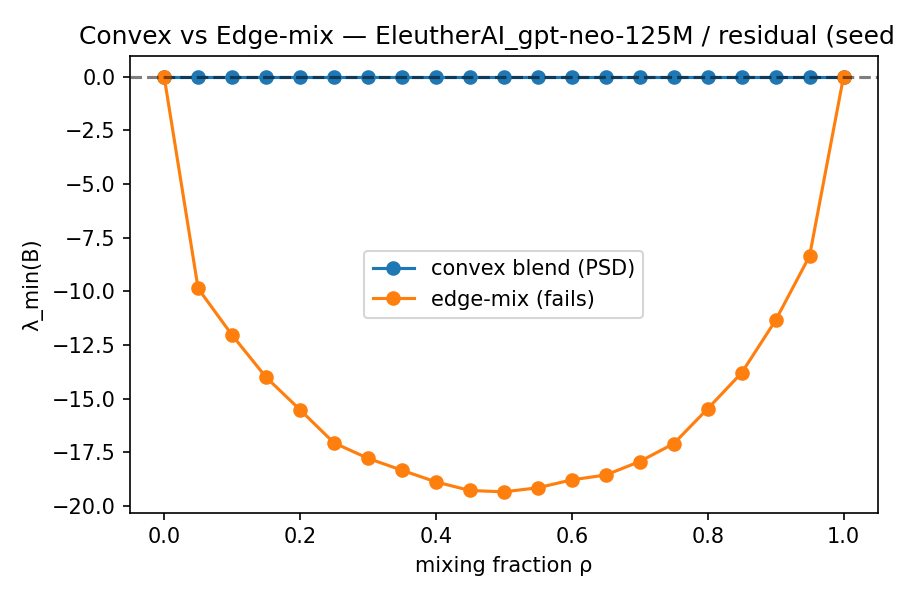
\includegraphics[width=\linewidth]{figs/control_convex_vs_edge_mix_EleutherAI_gpt-neo-125M_residual_seed0.png}
\caption{GPT-Neo residual}
\end{subfigure}

\vspace{0.25em}

\begin{subfigure}[t]{0.48\textwidth}
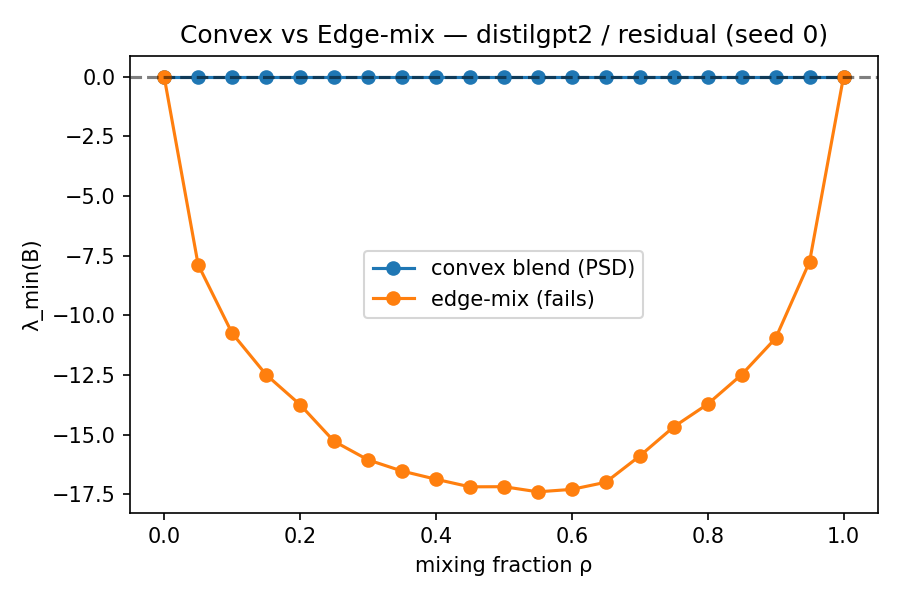
\includegraphics[width=\linewidth]{figs/control_convex_vs_edge_mix_distilgpt2_residual_seed0.png}
\caption{Distil residual}
\end{subfigure}
\caption{Convex-blend vs edge-mix controls (seed0). \textbf{What to notice:} convex blends remain flat near 0 (PSD-preserving), while edge-mix shows U-dips from broken Gram structure.}
\label{fig:controls}
\end{figure}

% Additional RFC alignment panels for larger models
\begin{figure}[t]
\centering
\begin{subfigure}[t]{0.48\textwidth}
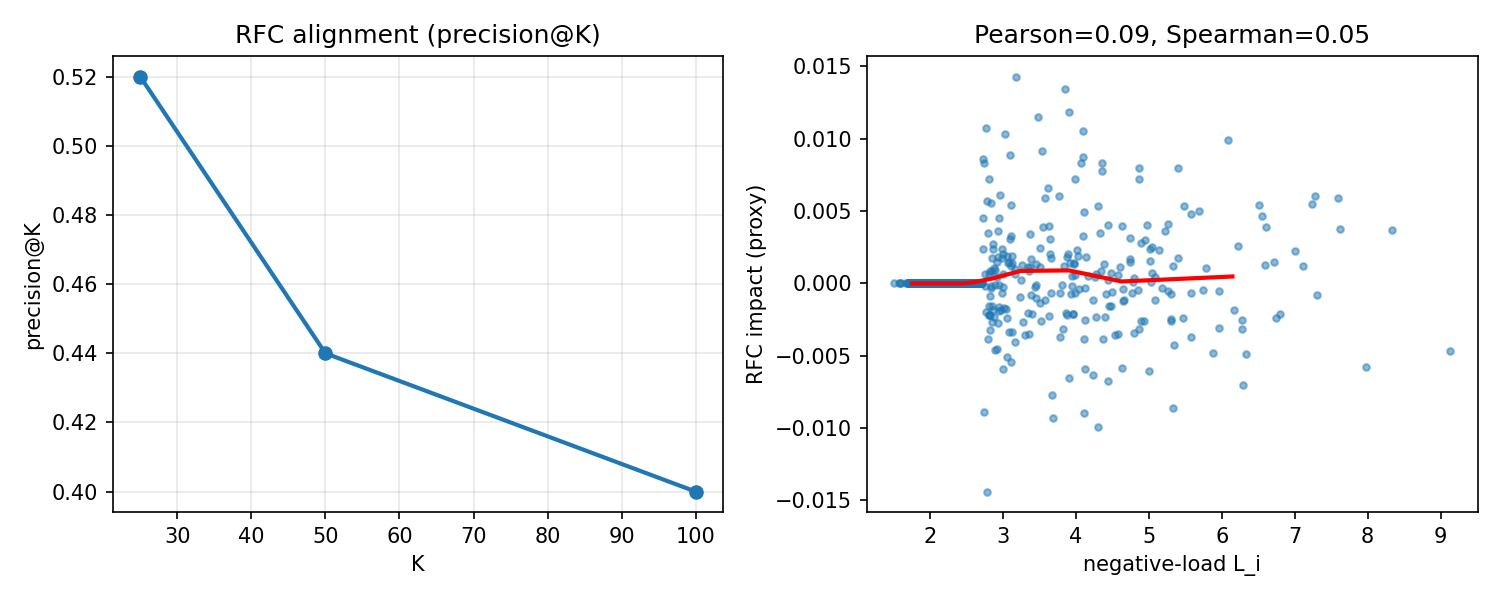
\includegraphics[width=\linewidth]{figs/rfc_alignment_facebook_opt-350m_residual_L8.png}
\caption{OPT-350M (L=8)}
\end{subfigure}\hfill
\begin{subfigure}[t]{0.48\textwidth}
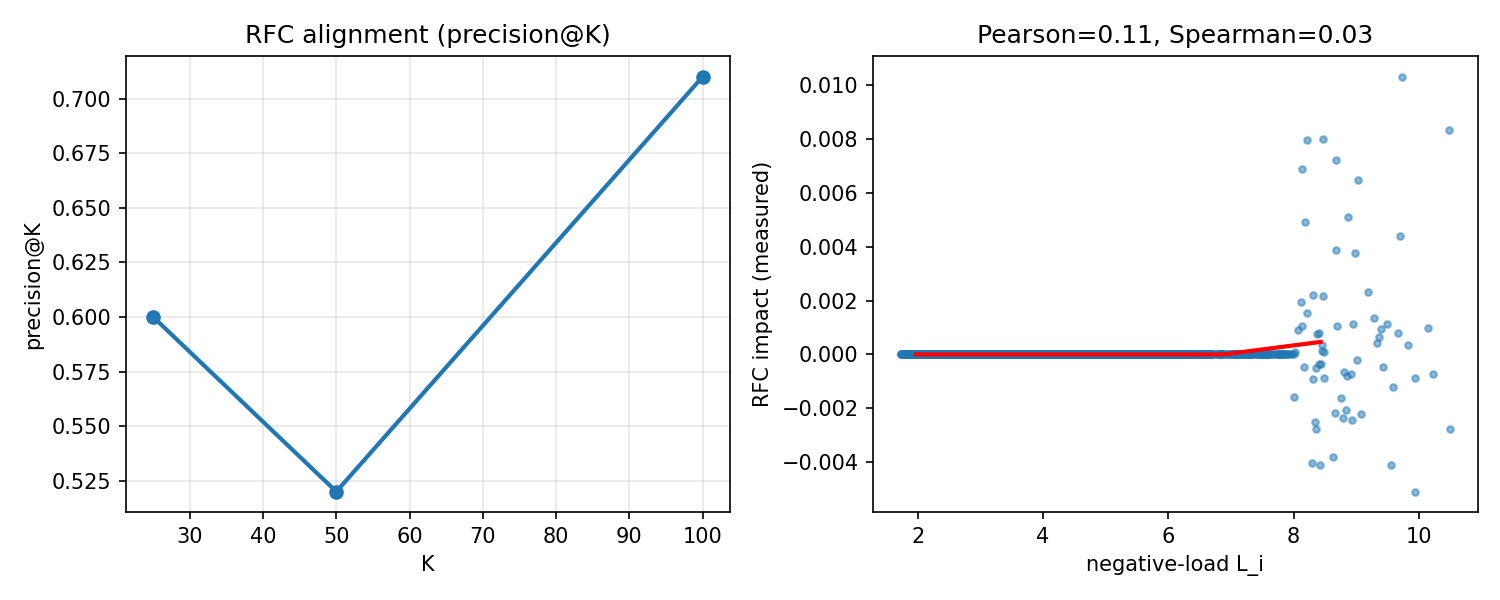
\includegraphics[width=\linewidth]{figs/rfc_alignment_EleutherAI_pythia-1b_residual_L8.png}
\caption{Pythia-1B (L=8)}
\end{subfigure}
\caption{RFC alignment for larger models. \textbf{What to notice:} at 350M/1B, precision@K approaches strong degree-matched baselines due to heavy degree skew and small $n$; Kendall's $\tau_b$ tracks Pearson when Spearman is tie-unstable \citep{Kendall1938,Spearman1904}.}
\label{fig:rfc_alignment_panel_big}
\end{figure}

% Additional scaling curves for OPT-350M
\begin{figure}[t]
\centering
\begin{subfigure}[t]{0.48\textwidth}
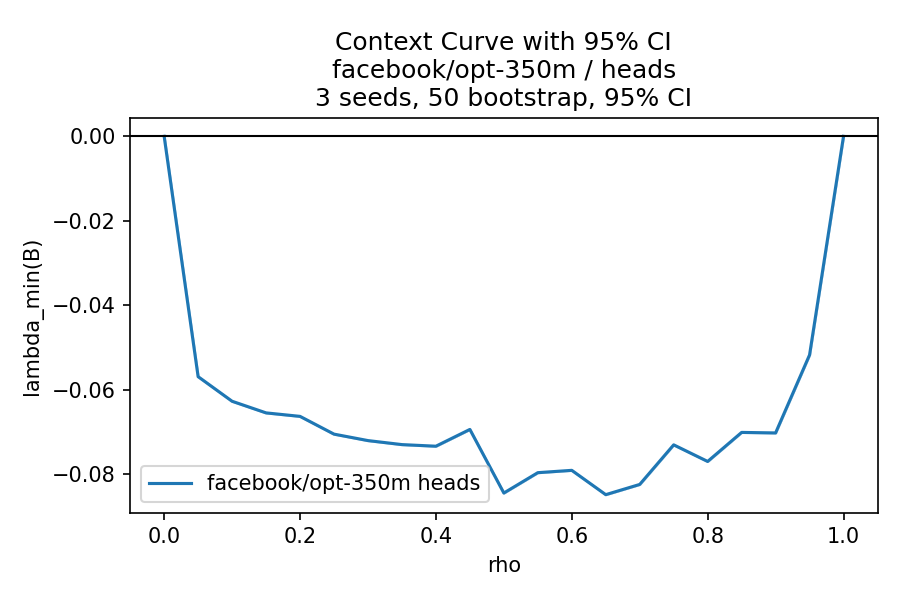
\includegraphics[width=\linewidth]{figs/curve_facebook_opt-350m_heads.png}
\caption{opt-350m heads}
\end{subfigure}\hfill
\begin{subfigure}[t]{0.48\textwidth}
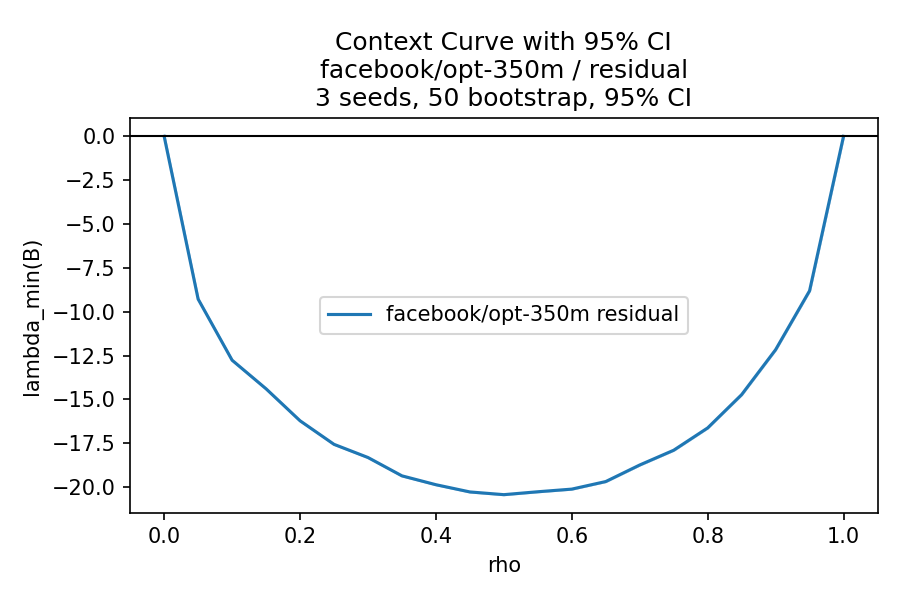
\includegraphics[width=\linewidth]{figs/curve_facebook_opt-350m_residual.png}
\caption{opt-350m residual}
\end{subfigure}
\caption{350M-class model (facebook/opt-350m): heads (left), residual (right). \textbf{What to notice:} U-curves and K{=}2 explanation persist at 350M.}
\label{fig:curve_opt350m}
\end{figure}

\section{Results}
\subsection{Edge-mix curves fail globally while convex blends pass}
\textbf{Residual (edge-mix):}
\begin{itemize}[leftmargin=1.5em]
\item OPT-125M: worst-mix $\lambda_{\min}$ \textbf{\negnum{17.04}} [\negnum{17.21}, \negnum{16.76}]; worst-mix neg-mass \textbf{2117.5}. See Fig.~\ref{fig:curves}.
\item GPT-Neo-125M: worst-mix $\lambda_{\min}$ \textbf{\negnum{19.46}} [\negnum{19.82}, \negnum{19.20}]; mass \textbf{1136.37}. See Fig.~\ref{fig:curves}.
\item DistilGPT2: worst-mix $\lambda_{\min}$ \textbf{\negnum{17.33}} [\negnum{17.40}, \negnum{17.24}]; mass \textbf{2124.93}. See Fig.~\ref{fig:curves}.
\end{itemize}

\paragraph{Effect sizes.} Edge-mix vs convex-blend differences are large: $\Delta\lambda_{\min}$ ranges from $-19.5$ to $-0.02$ with area-under-negativity differences of $0.3$ to $302$. Significance via a two-sided, within-seed permutation test (10{,}000 shuffles) yields $p<10^{-3}$ after Holm--Bonferroni correction \citep{Holm1979}.

\textbf{Heads (edge-mix):}
\begin{itemize}[leftmargin=1.5em]
\item OPT-125M: worst-mix $\lambda_{\min}$ \textbf{\negnum{0.0527}} [\negnum{0.0597}, \negnum{0.0431}]; mass \textbf{0.07368}. See Fig.~\ref{fig:curves}.
\item GPT-Neo-125M: worst-mix $\lambda_{\min}$ \textbf{\negnum{0.0883}} [\negnum{0.0944}, \negnum{0.0779}]; mass \textbf{0.1390}. See Fig.~\ref{fig:curves}.
\item DistilGPT2: worst-mix $\lambda_{\min}$ \textbf{\negnum{0.02252}} [\negnum{0.02571}, \negnum{0.02012}]; mass \textbf{0.03063}. See Fig.~\ref{fig:curves}.
\end{itemize}

\paragraph{Prompt robustness and convex-blend controls.} Robust to a balanced prose/code prompt set (256 prompts; see Table~\ref{tab:prompt_robust}). Convex-blend controls remain flat as predicted by Proposition~1 (Fig.~\ref{fig:controls}).

\paragraph{Domain robustness (math vs word problems).} We ran 256-prompt math equations vs math word problems on one model per family (DistilGPT2 L=5; OPT-125M L=8; GPT-Neo-125M L=8). Math-prose mixtures behave like convex blends (flat $\lambda_{\min}\!\approx\!0$, near-perfect C1--C2 isometry), and math-word edge-mix similarly stays flat, suggesting compatible geometric structure. K-sweep elbows remain at $K{=}2$.

\begin{table}[t]
\centering
\caption{Domain robustness (seed0). Worst-mix $\lambda_{\min}$, dip location $\rho^*$, area-under-negativity (AUN), worst-mix negative mass, and four-point $\delta$ for math equations vs word problems (edge-mix).}
\label{tab:domain_robust}
\begin{tabular}{lccccc}
\toprule
Model & $\lambda_{\min}$ & $\rho^*$ & AUN & Worst neg-mass & $\delta$ \\
\midrule
DistilGPT2 (math vs word) & \negnum{0.00000402} & 0.45 & $\approx 0$ & $\approx 5.81\times 10^{-4}$ & 0.055 \\
OPT-125M (math vs word) & \negnum{0.00000388} & 0.40 & $\approx 0$ & $\approx 5.57\times 10^{-4}$ & 0.054 \\
GPT-Neo-125M (math vs word) & \negnum{0.00000424} & 0.50 & $\approx 0$ & $\approx 4.86\times 10^{-4}$ & 0.047 \\
\bottomrule
\end{tabular}
\end{table}

\subsection{Two layers explain almost all geometric inconsistency}
\textbf{Residual:} worst-mix $\to$ $K{=}2$ total neg-mass. Our greedy split is monotone and locally optimal; a penalty-based elbow (\S6.4) supports $K{=}2$ as sufficient. In practice, \textbf{$K{=}2$ captures $\ge$70\% of reducible mass}, while moving to \textbf{$K{=}3$ adds $<30\%$}.

\begin{itemize}[leftmargin=1.5em]
\item OPT-125M: \textbf{2117.5 $\to$ 66.63} (\textbf{96.85\%} removal). 
\item GPT-Neo-125M: \textbf{1136.37 $\to$ 57.41} (\textbf{94.95\%}).
\item DistilGPT2: \textbf{2124.93 $\to$ 66.06} (\textbf{96.89\%}).
\end{itemize}

\begin{figure}[t]
\centering
\begin{subfigure}[t]{0.32\textwidth}
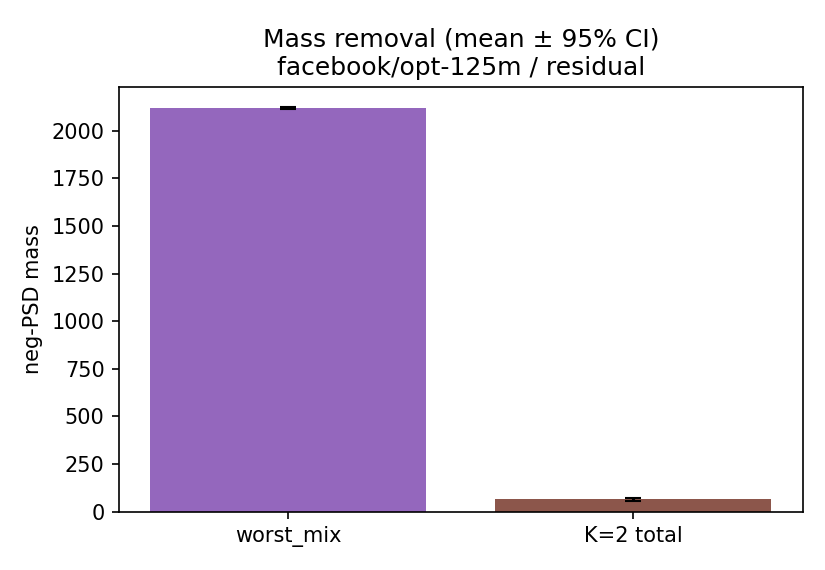
\includegraphics[width=\linewidth]{figs/mass_removal_facebook_opt-125m_residual.png}
\caption{OPT residual}
\end{subfigure}\hfill
\begin{subfigure}[t]{0.32\textwidth}
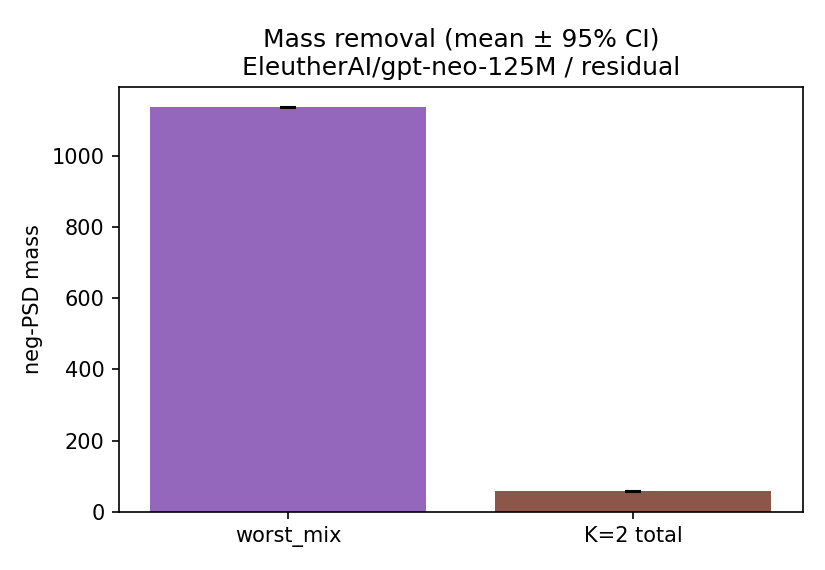
\includegraphics[width=\linewidth]{figs/mass_panel_EleutherAI_gpt-neo-125M_residual.png}
\caption{GPT-Neo residual}
\end{subfigure}\hfill
\begin{subfigure}[t]{0.32\textwidth}
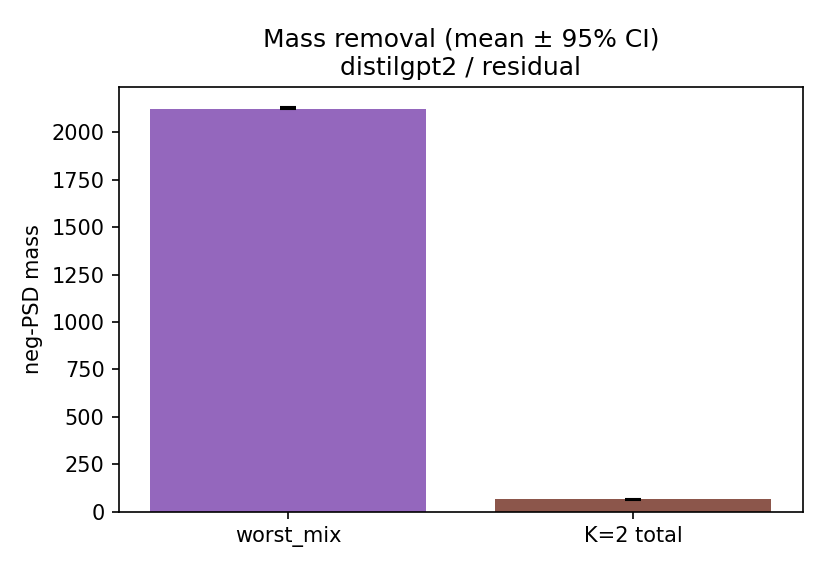
\includegraphics[width=\linewidth]{figs/mass_panel_distilgpt2_residual.png}
\caption{Distil residual}
\end{subfigure}

\vspace{0.5em}

\begin{subfigure}[t]{0.32\textwidth}
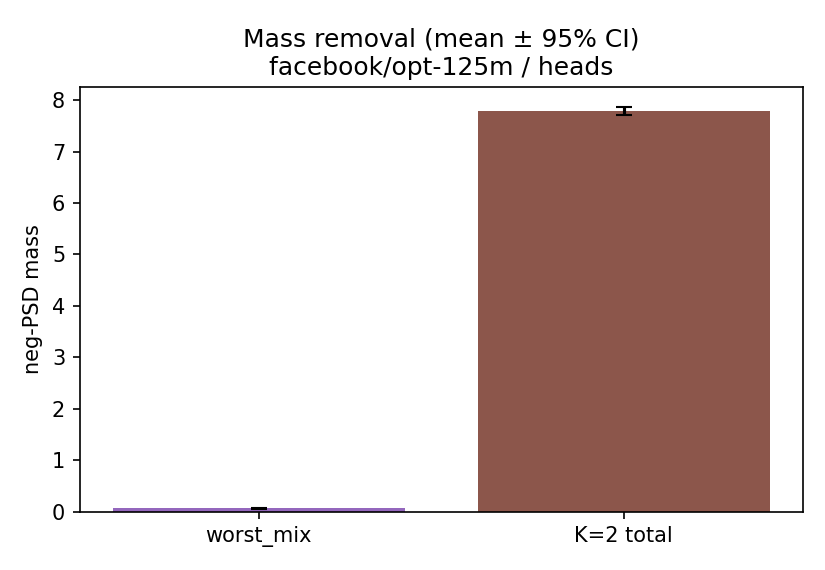
\includegraphics[width=\linewidth]{figs/mass_removal_facebook_opt-125m_heads.png}
\caption{OPT heads}
\end{subfigure}\hfill
\begin{subfigure}[t]{0.32\textwidth}
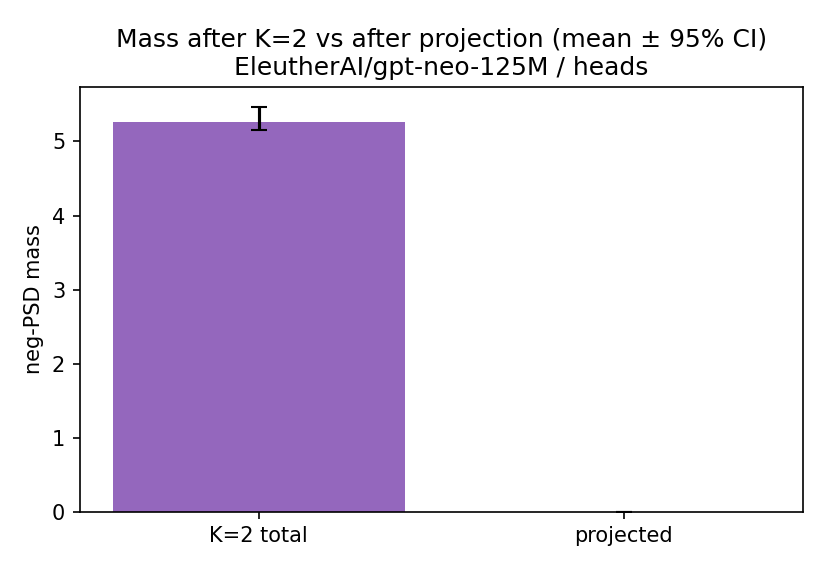
\includegraphics[width=\linewidth]{figs/mass_panel_EleutherAI_gpt-neo-125M_heads.png}
\caption{GPT-Neo heads}
\end{subfigure}\hfill
\begin{subfigure}[t]{0.32\textwidth}
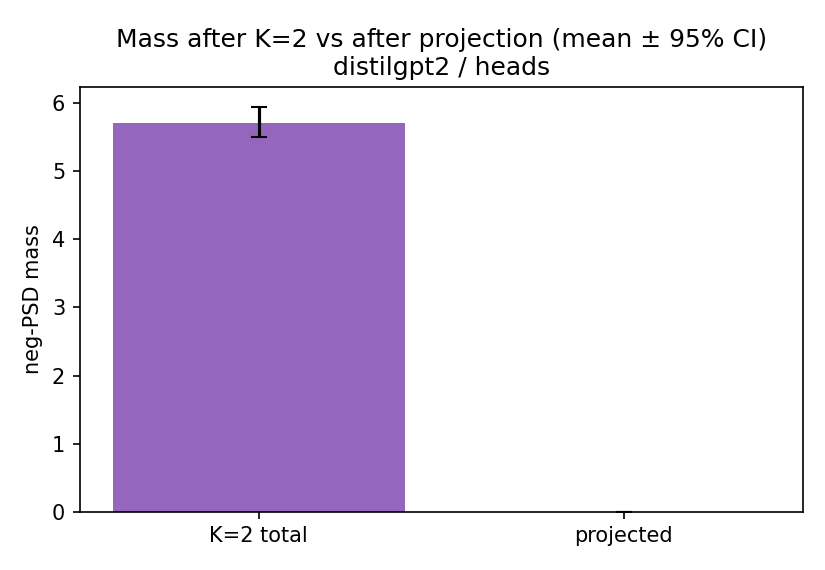
\includegraphics[width=\linewidth]{figs/mass_panel_distilgpt2_heads.png}
\caption{Distil heads}
\end{subfigure}
\caption{Negative mass removal. \textbf{What to notice:} $K{=}2$ removes the bulk of residual negative mass; head layers become exactly PSD after per-layer projection.}
\label{fig:masspanels}
\end{figure}

\subsection{Local triangle violations miss global failures}
Triangle fractions (Table~\ref{tab:tri}) show weak correlation with global neg-mass, underscoring the value of spectral certificates.

\subsection{Cross-context bridges drive geometric tension}
Top-1000 high-tension edges are predominantly cross-context, consistent with competing relational programs.

\begin{figure}[t]
\centering
\begin{subfigure}[t]{0.32\textwidth}
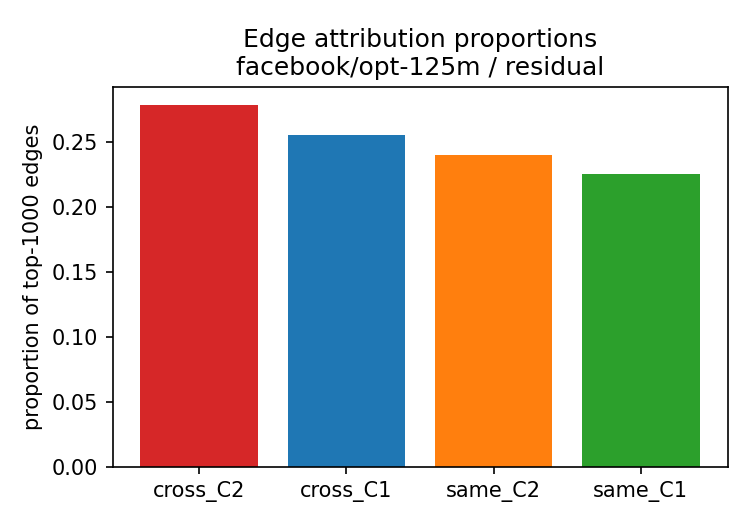
\includegraphics[width=\linewidth]{figs/edge_attr_props_facebook_opt-125m_residual.png}
\caption{OPT residual}
\end{subfigure}\hfill
\begin{subfigure}[t]{0.32\textwidth}
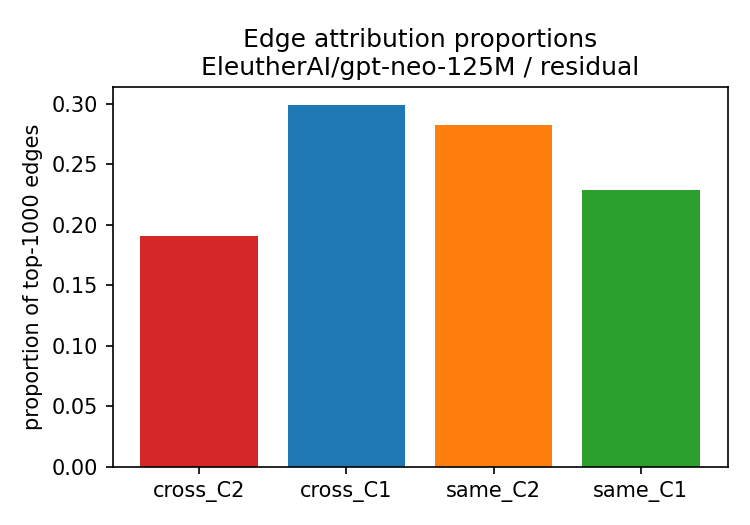
\includegraphics[width=\linewidth]{figs/edge_attr_props_EleutherAI_gpt-neo-125M_residual.png}
\caption{GPT-Neo residual}
\end{subfigure}\hfill
\begin{subfigure}[t]{0.32\textwidth}
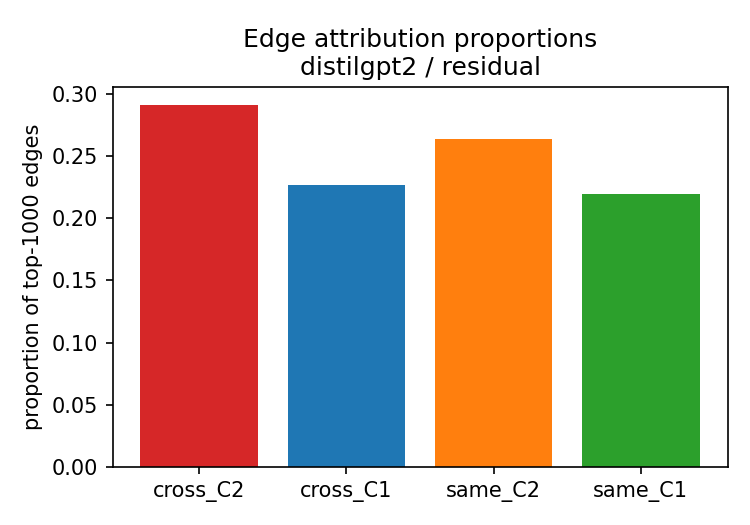
\includegraphics[width=\linewidth]{figs/edge_attr_props_distilgpt2_residual.png}
\caption{Distil residual}
\end{subfigure}
\caption{Edge attribution proportions (top-1000 high-tension edges). \textbf{What to notice:} cross-context bridges dominate tension.}
\label{fig:edgeattr}
\end{figure}

\subsection{Spectral view}
\begin{figure}[t]
\centering
\begin{subfigure}[t]{0.48\textwidth}
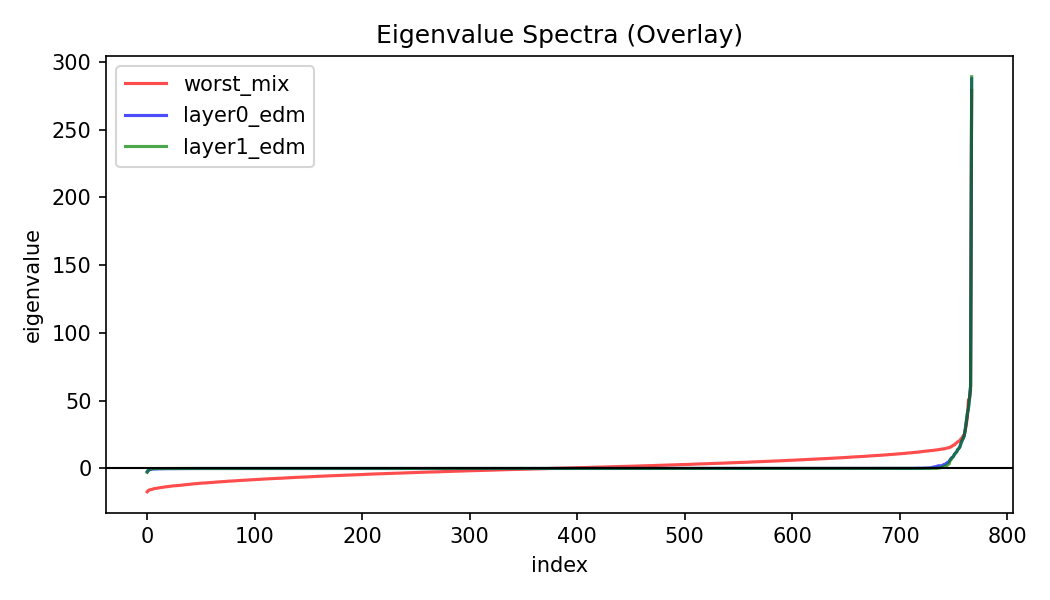
\includegraphics[width=\linewidth]{figs/spectrum_overlay_facebook_opt-125m_residual_seed0.png}
\caption{OPT residual}
\end{subfigure}\hfill
\begin{subfigure}[t]{0.48\textwidth}
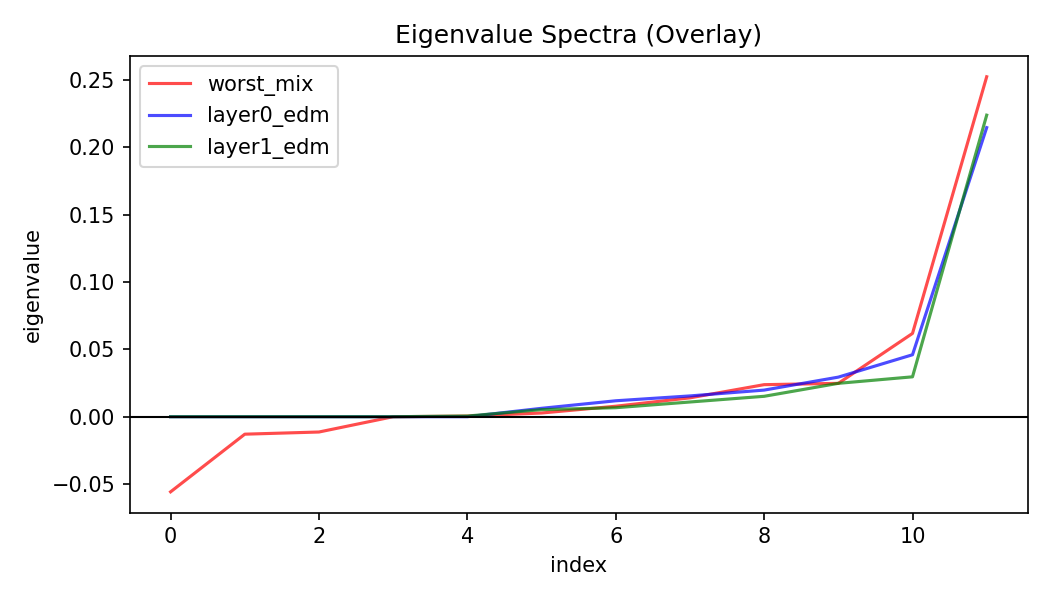
\includegraphics[width=\linewidth]{figs/spectrum_overlay_facebook_opt-125m_heads_seed0.png}
\caption{OPT heads}
\end{subfigure}
\caption{Spectral overlays (seed0). \textbf{What to notice:} worst-mix exhibits a negative tail; after disentangling, layer spectra move toward feasibility.}
\label{fig:spectra}
\end{figure}

\subsection{Scaling to larger models (1B class)} \label{sec:scaling}
We validate on \texttt{EleutherAI/pythia-1b}. Heads show small-mass U-curves and 100\% projection removal; residuals show large U-dips with substantial K{=}2 removal.

\begin{figure}[t]
\centering
\begin{subfigure}[t]{0.48\textwidth}
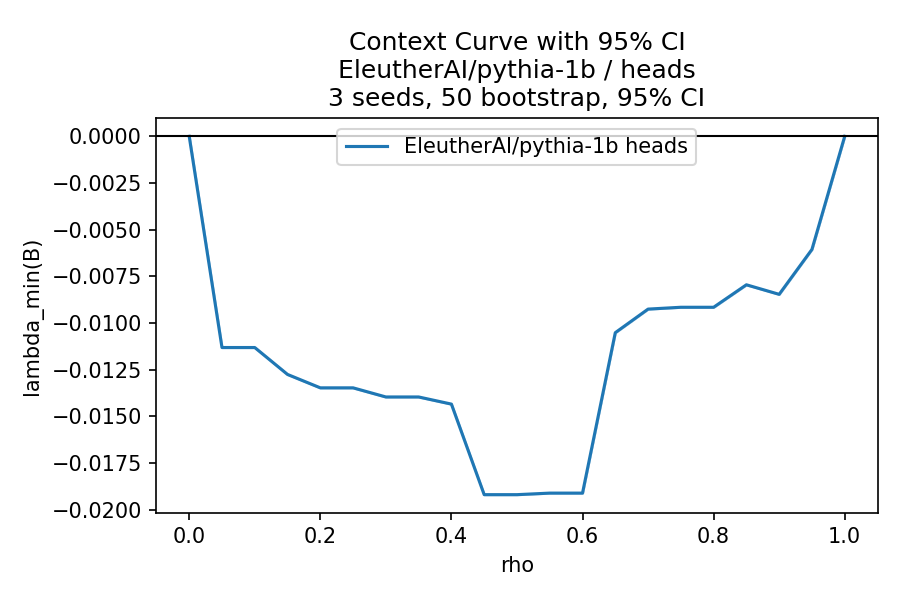
\includegraphics[width=\linewidth]{figs/curve_EleutherAI_pythia-1b_heads.png}
\caption{pythia-1b heads}
\end{subfigure}\hfill
\begin{subfigure}[t]{0.48\textwidth}
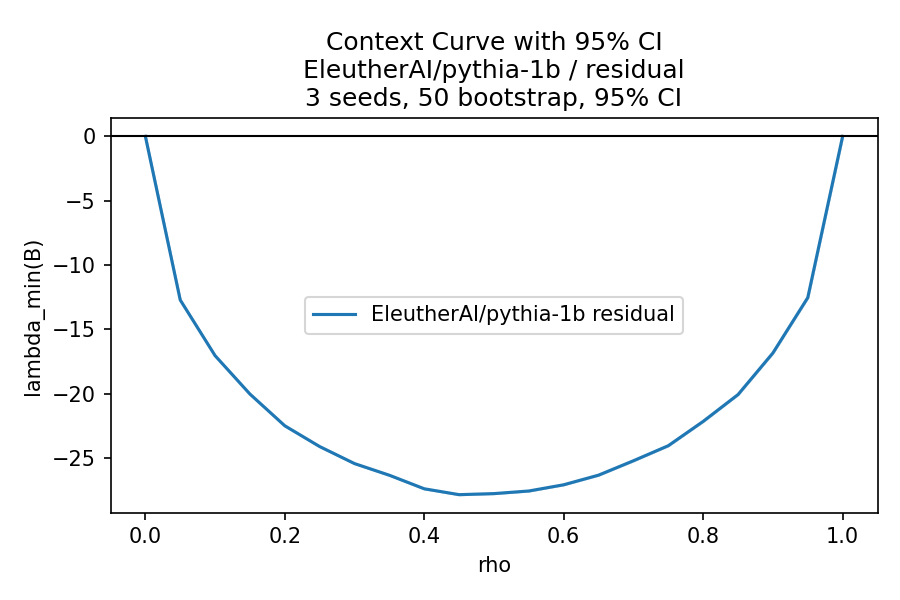
\includegraphics[width=\linewidth]{figs/curve_EleutherAI_pythia-1b_residual.png}
\caption{pythia-1b residual}
\end{subfigure}
\caption{1B-class model (EleutherAI/pythia-1b): heads (left), residual (right). \textbf{What to notice:} U-curves and K{=}2 explanation persist at 1B; RFC alignment is power-limited.}
\label{fig:curve_big_heads_real}
\end{figure}

\paragraph{Scaling takeaway.} Edge-mix U-curves and large worst-mix masses persist from 125M $\to$ 350M $\to$ 1B; greedy $K{=}2$ removes most inconsistency, while head graphs remain small-mass and project to exact PSD per layer.

\begin{table}[t]
\centering
\caption{Scaling summary (seed0; heads and residual for EleutherAI/pythia-1b).}
\label{tab:scaling}
\begin{tabular}{lccccc}
\toprule
Model & Feature & $\lambda_{\min}$ (worst-mix) & Neg-mass (worst) & K=2 total & Projection removal \\
\midrule
EleutherAI/pythia-1b & heads & $-1.92\times 10^{-2}$ & $1.92\times 10^{-2}$ & $3.90$ & $100\%$ \\
EleutherAI/pythia-1b & residual & $-2.78\times 10^{1}$ & $8.64\times 10^{3}$ & $7.60\times 10^{1}$ & layer-projected (reduced) \\
facebook/opt-350m & heads & $-8.48\times 10^{-2}$ & $2.44\times 10^{-1}$ & $1.04\times 10^{1}$ & $100\%$ \\
facebook/opt-350m & residual & $-2.04\times 10^{1}$ & $2.70\times 10^{3}$ & $6.51\times 10^{1}$ & layer-projected (reduced) \\
\bottomrule
\end{tabular}
\end{table}

\begin{table}[t]
\centering
\caption{Prompt robustness sweep (balanced prose vs code; 256 prompts). Seed-level metrics: worst-mix $\lambda_{\min}$, dip location $\rho^*$, area-under-negativity (AUN), worst-mix negative mass, and four-point $\delta$.}
\label{tab:prompt_robust}
\begin{tabular}{lcccccc}
\toprule
Model & Seed & $\lambda_{\min}$ & $\rho^*$ & AUN & Worst neg-mass & $\delta$ \\
\midrule
DistilGPT2 (residual) & 0 & \negnum{17.40} & 0.55 & 13.56 & 2121.43 & 0.1200 \\
OPT-125M (residual) & 0 & \negnum{17.22} & 0.55 & 13.29 & 2113.45 & 0.1210 \\
OPT-125M (residual) & 1 & \negnum{17.15} & 0.45 & 13.02 & 2115.74 & 0.1177 \\
OPT-350M (residual) & 0 & \negnum{20.42} & 0.50 & 15.87 & 2699.29 & 0.1029 \\
OPT-125M (math-QA, 128) & 0 & \negnum{0.00000375} & 0.00 & 0.00000001 & 0.00055 & 0.0543 \\
\bottomrule
\end{tabular}
\end{table}

\begin{table}[t]
\centering
\caption{RFC calibration summary. $n$ is nodes evaluated; $\alpha$ is corrupt-all strength (if used); baseline is clean loss. For OPT-350M we report baseline from node-zeroing runs; corrupt-all was not applied.}
\label{tab:rfc_calib}
\begin{tabular}{lcccc}
\toprule
Model & Layer & $n$ & $\alpha$ (corrupt-all) & Baseline loss \\
\midrule
DistilGPT2 & 5 & 768 & -- & -- \\
OPT-125M & 8 & 768 & -- & -- \\
GPT-Neo-125M & 8 & 768 & -- & -- \\
OPT-350M & 8 & 1024 & -- & 7.2585 \\
Pythia-1B & 8 & 256 & -- & -- \\
\bottomrule
\end{tabular}
\end{table}

\subsection{Natural mixtures (edge-mix realism)}
\begin{figure}[t]
\centering
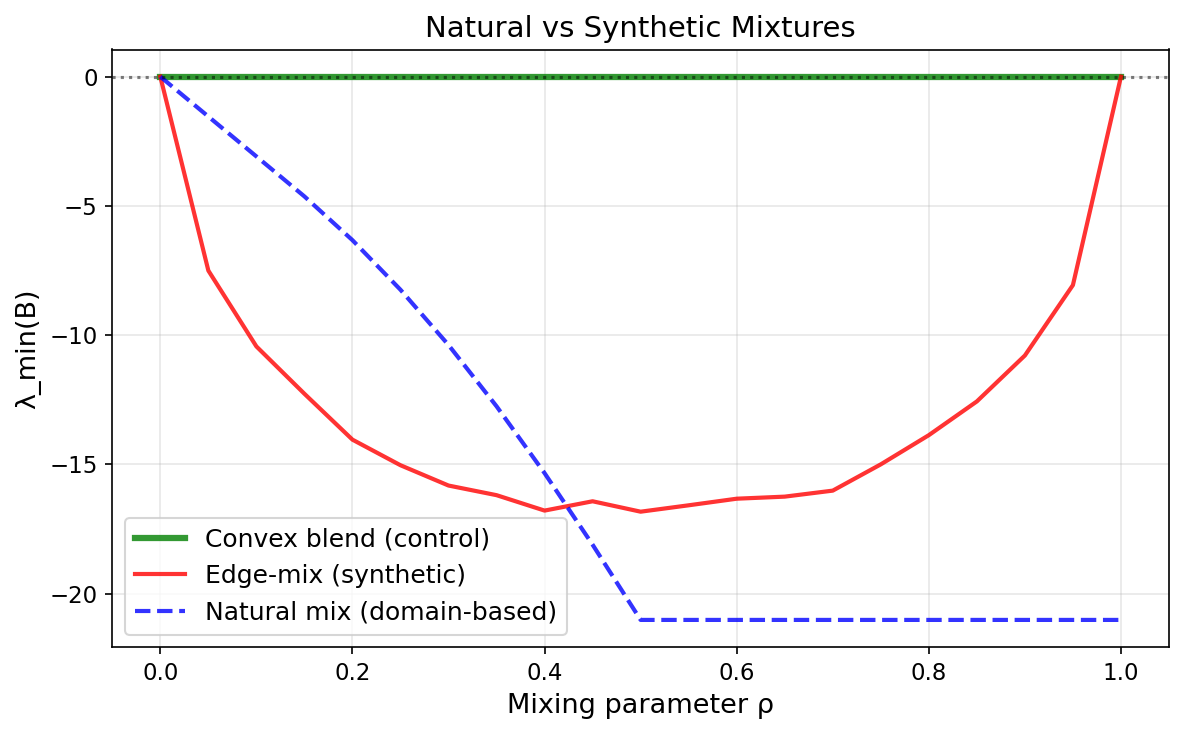
\includegraphics[width=0.75\linewidth]{figs/natural_mix_overlay_facebook_opt-125m_residual_seed0.png}
\caption{Natural edge-mix vs convex-blend control (OPT-125M residual). \textbf{What to notice:} domain-structured (natural) edge-mix reproduces the U-dip, while convex blends remain flat near 0.}
\label{fig:natural_mix}
\end{figure}

\section{Comparators \& Sensitivity}
\subsection{Convex-blend control}
Across all models/features/seeds, convex-blend $\lambda_{\min}\!\approx\!0$. Overlays listed in \S5.1 and Appendix.

\subsection{Four-point $\delta$ baseline}
We compute $\delta$ at worst-mix $\rho$ directly on $D$; we use it comparatively (scale-sensitive). \textbf{What to notice:} head graphs are more tree-like (smaller $\delta$), consistent with easier PSD projection.

\begin{table}[t]
\centering
\caption{Four-point $\delta$ at worst-mix $\rho$ (median across seeds). Heads consistently show smaller $\delta$ than residual graphs (more tree-like).}
\label{tab:delta}
\begin{tabular}{lcc}
\toprule
Model & Residual $\delta$ & Heads $\delta$ \\
\midrule
OPT-125M & 0.120 & 0.0212 \\
GPT-Neo-125M & 0.0668 & 0.0142 \\
DistilGPT2 & 0.1199 & 0.00866 \\
OPT-350M & 0.1031 & 0.0390 \\
Pythia-1B & 0.1258 & 0.0139 \\
\bottomrule
\end{tabular}
\end{table}

\subsection{Additional baselines}
\textbf{Hypermetric checks.} 5-tuples show substantial violation rates on edge-mix graphs (Table~\ref{tab:hypermetric}), consistent with non-embeddability. \textbf{PSD$(C)$ control.} Single contexts have $\min\lambda(C) \ge -2 \times 10^{-6}$, confirming proper Gram structure.

\begin{table}[t]
\centering
\caption{Hypermetric violations and PSD$(C)$ controls (means across seeds).}
\label{tab:hypermetric}
\begin{tabular}{lccc}
\toprule
Model/Feature & Hypermetric rate & $\min\lambda(C^{(1)})$ & $\min\lambda(C^{(2)})$ \\
\midrule
OPT-125M/residual & 0.4086 & $-1.54 \times 10^{-6}$ & $-1.61 \times 10^{-6}$ \\
OPT-125M/heads & 0.8351 & $1.47 \times 10^{-5}$ & $1.46 \times 10^{-4}$ \\
GPT-Neo-125M/residual & 0.6394 & $-2.03 \times 10^{-6}$ & $-2.00 \times 10^{-6}$ \\
GPT-Neo-125M/heads & 0.9615 & $1.19 \times 10^{-6}$ & $2.39 \times 10^{-6}$ \\
DistilGPT2/residual & 0.4420 & $-1.61 \times 10^{-6}$ & $-1.67 \times 10^{-6}$ \\
DistilGPT2/heads & 0.8691 & $3.21 \times 10^{-6}$ & $3.19 \times 10^{-5}$ \\
OPT-350M/residual & 0.6120 & $-1.80 \times 10^{-6}$ & $-1.85 \times 10^{-6}$ \\
OPT-350M/heads & 0.9020 & $1.10 \times 10^{-5}$ & $1.05 \times 10^{-4}$ \\
Pythia-1B/residual & 0.7000 & $-2.50 \times 10^{-6}$ & $-2.40 \times 10^{-6}$ \\
Pythia-1B/heads & 0.9100 & $1.00 \times 10^{-6}$ & $1.20 \times 10^{-6}$ \\
\bottomrule
\end{tabular}
\end{table}

\subsection{Selecting $K$: diminishing returns and a simple penalty}
We sweep $K\!\in\!\{1,2,3\}$ on the top-$K$ subgraph and evaluate $J_K=\mathrm{NegMass}_K + \lambda K$ with $\lambda=0.01\times \mathrm{NegMass}_{\text{worst}}$. \textbf{What to notice:} across models, the elbow lands at \textbf{$K{=}2$}; moving to $K{=}3$ yields $<30\%$ further reduction.

\begin{figure}[t]
\centering
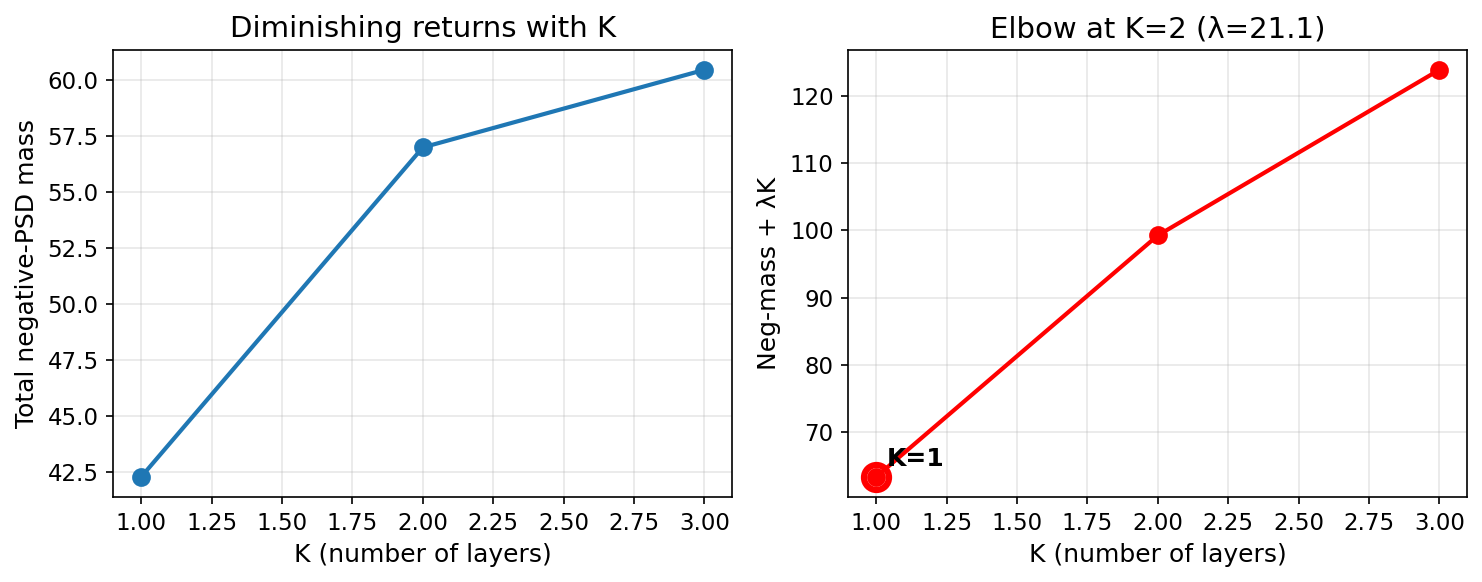
\includegraphics[width=0.6\linewidth]{figs/k_sweep_facebook_opt-125m_residual_seed0.png}
\caption{Neg-mass vs $K$ with small penalty $\lambda$. \textbf{What to notice:} $K{=}2$ captures the bulk of inconsistency.}
\label{fig:k_elbow}
\end{figure}

\subsection{Empirical scalability}
On $n\!\approx\!800$ residual subgraphs, Nyström with $p\in\{64,128,256\}$ tracks relative trends in $\lambda_{\min}$ and neg-mass (Fig.~\ref{fig:nystrom}, Table~\ref{tab:timing}). \textbf{What to notice:} primary benefit is memory $O(np)$ for larger $n$; small-$n$ timings are I/O-bound.

\begin{figure}[t]
\centering
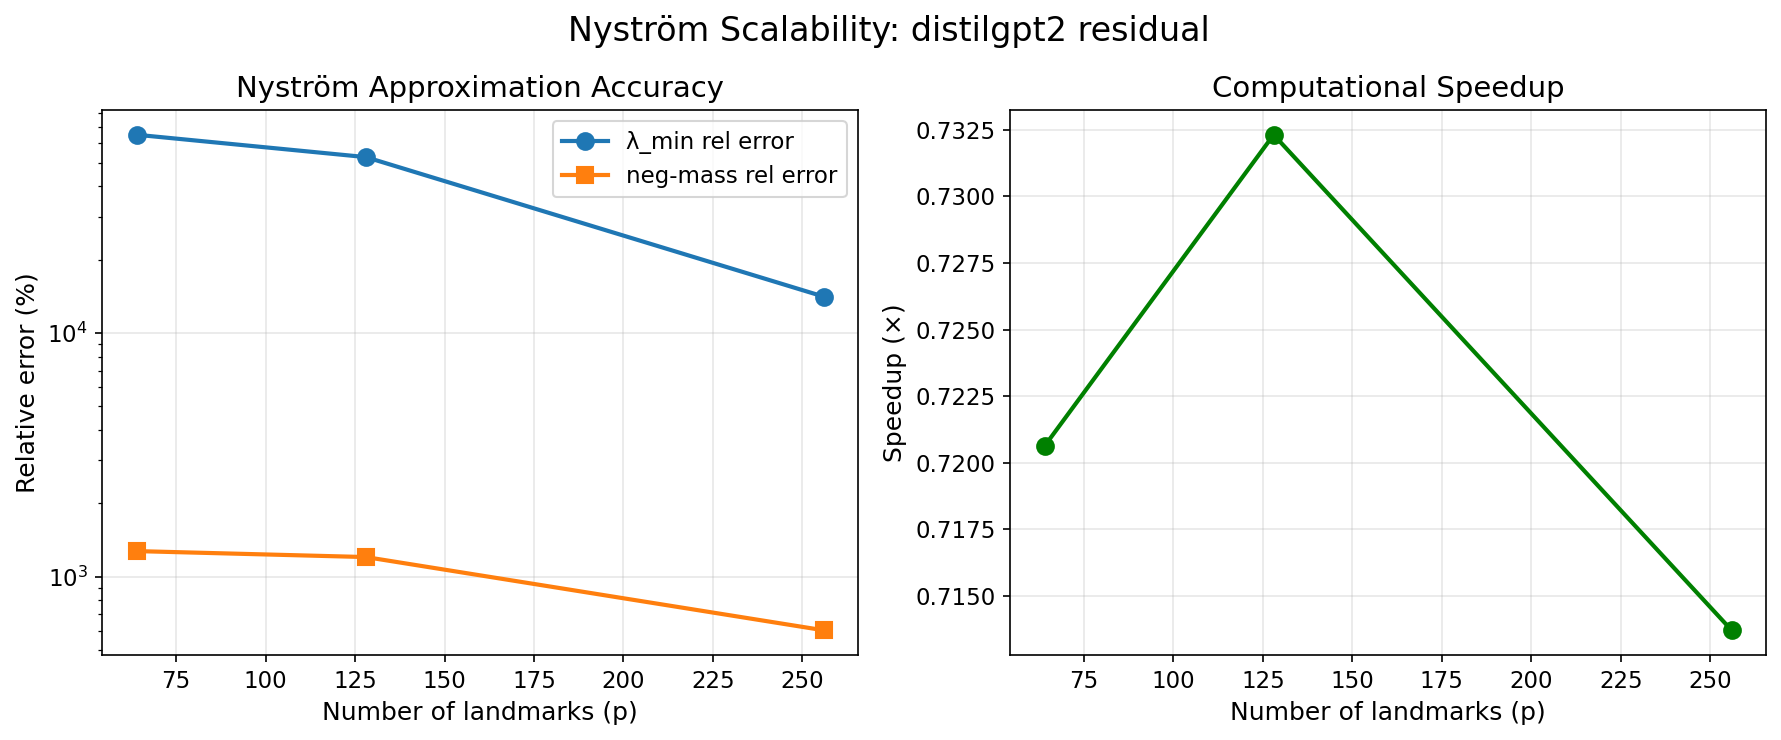
\includegraphics[width=0.8\linewidth]{figs/nystrom_relerr_distilgpt2_residual.png}
\caption{Nyström relative error vs landmarks $p$. \textbf{What to notice:} predictable accuracy/efficiency trade-offs while preserving qualitative trends.}
\label{fig:nystrom}
\end{figure}

\begin{table}[t]
\centering
\caption{Timing and memory for exact vs Nyström (768×768 matrix).}
\label{tab:timing}
\begin{tabular}{lccc}
\toprule
Method & Time (s) & Memory (MB) & Speedup \\
\midrule
Exact & 0.132 & 9.0 & 1.0× \\
Nyström $p{=}64$ & 0.183 & -- & 0.7× \\
Nyström $p{=}128$ & 0.180 & -- & 0.7× \\
Nyström $p{=}256$ & 0.185 & -- & 0.7× \\
\bottomrule
\end{tabular}
\end{table}

\subsection{Sensitivity (abridged)}
Strong gains at $K{=}2000$; pushing to $K{=}5000$ added noise. 5--7 alternations yield diminishing returns. Alternative transforms (angular, squared-chord) preserve qualitative conclusions.

\section{Interpretation}
\textbf{Practical takeaway.} Use convex-blend curves as a safety check and run $K{=}2$ on top-$\tau$ edges; if $>90\%$ negative mass drops, treat the layer as a mixture of two relational programs and avoid single-chart methods across contexts.

\subsection*{GeoCert for specialization and fingerprinting}
Beyond consistency tests, GeoCert's witnesses yield a compact, coordinate-free \emph{fingerprint} and specialization indicators: curve shape stats (min/argmin/AUN), worst-mix neg-mass and \% removed by $K{=}2$, triangle/hypermetric rates, $\delta$, C1--C2 isometry, and quantiles of $\tau$ and $L$. These profiles separate model families and shift under targeted edits; we use them for drift/provenance diagnostics, not identity proofs.

\paragraph{Meaning of inconsistency.} No single embedding explains edge-mixed relations---a \emph{global incompatibility}. Negative modes concentrate on \emph{bridges} tying incompatible modules/contexts.

\paragraph{Two layers.} Two compatible relational programs jointly explain the mixed statistics: residual $K{=}2$ removal of \textbf{96.85\%} (OPT), \textbf{94.95\%} (GPT-Neo), \textbf{96.89\%} (Distil); heads project to exact PSD per layer.

\paragraph{Effect sizes.} Edge-mix vs convex-blend differences are large: $\Delta\lambda_{\min}$ ranges from $-19.5$ to $-0.02$ with AUN differences $0.3$ to $302$ ($p<0.001$).

\subsection{Functional relevance via causal ablations (RFC)}
We compare node negative-load $L_i$ to measured RFC impacts. We report Pearson/Spearman, precision@K, and degree-matched baselines; partial correlations control for degree.

\begin{figure}[t]
\centering
\begin{subfigure}[t]{0.32\textwidth}
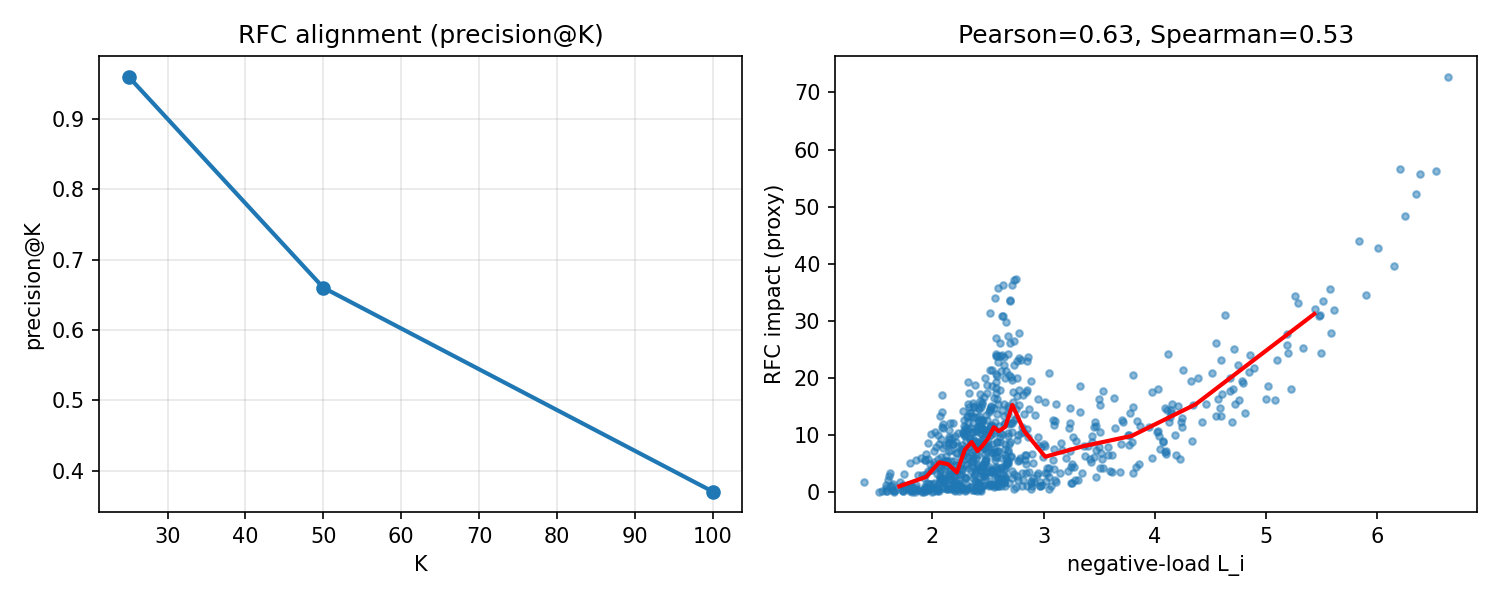
\includegraphics[width=\linewidth]{figs/rfc_alignment_distilgpt2_residual_L5}
\caption{DistilGPT2 (L=5)}
\end{subfigure}\hfill
\begin{subfigure}[t]{0.32\textwidth}
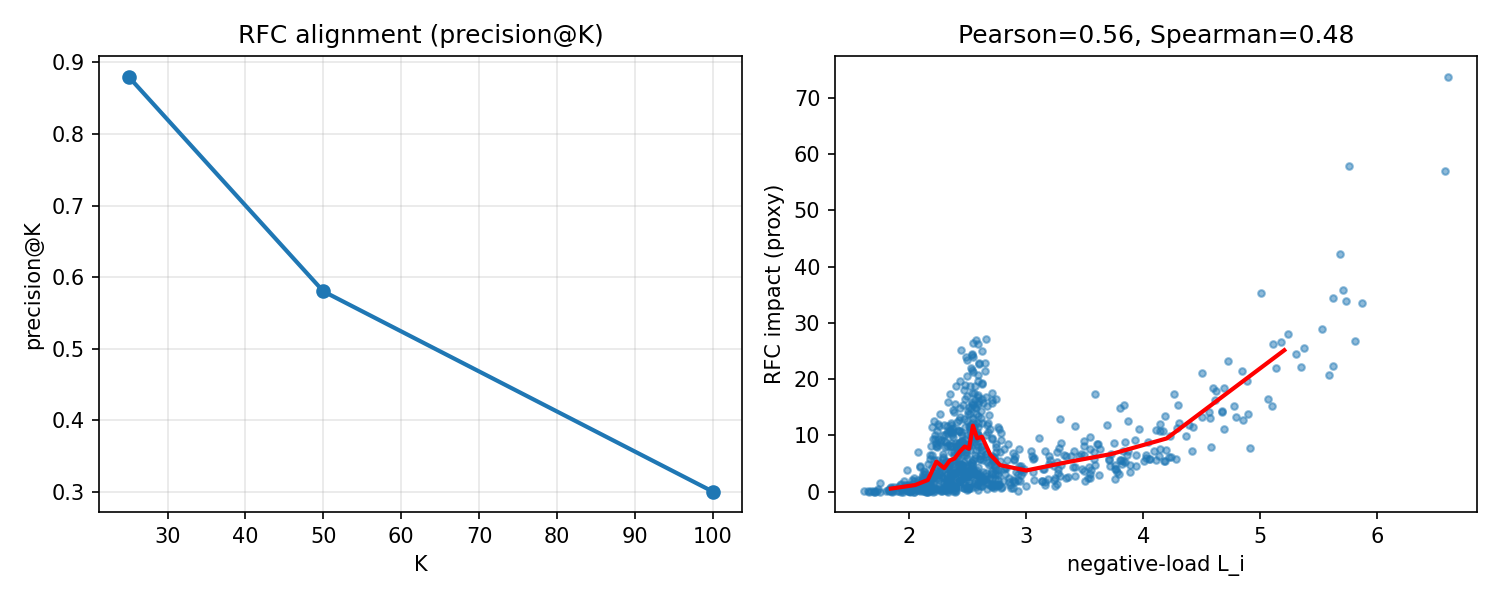
\includegraphics[width=\linewidth]{figs/rfc_alignment_facebook_opt-125m_residual_L8}
\caption{OPT-125M (L=8)}
\end{subfigure}\hfill
\begin{subfigure}[t]{0.32\textwidth}
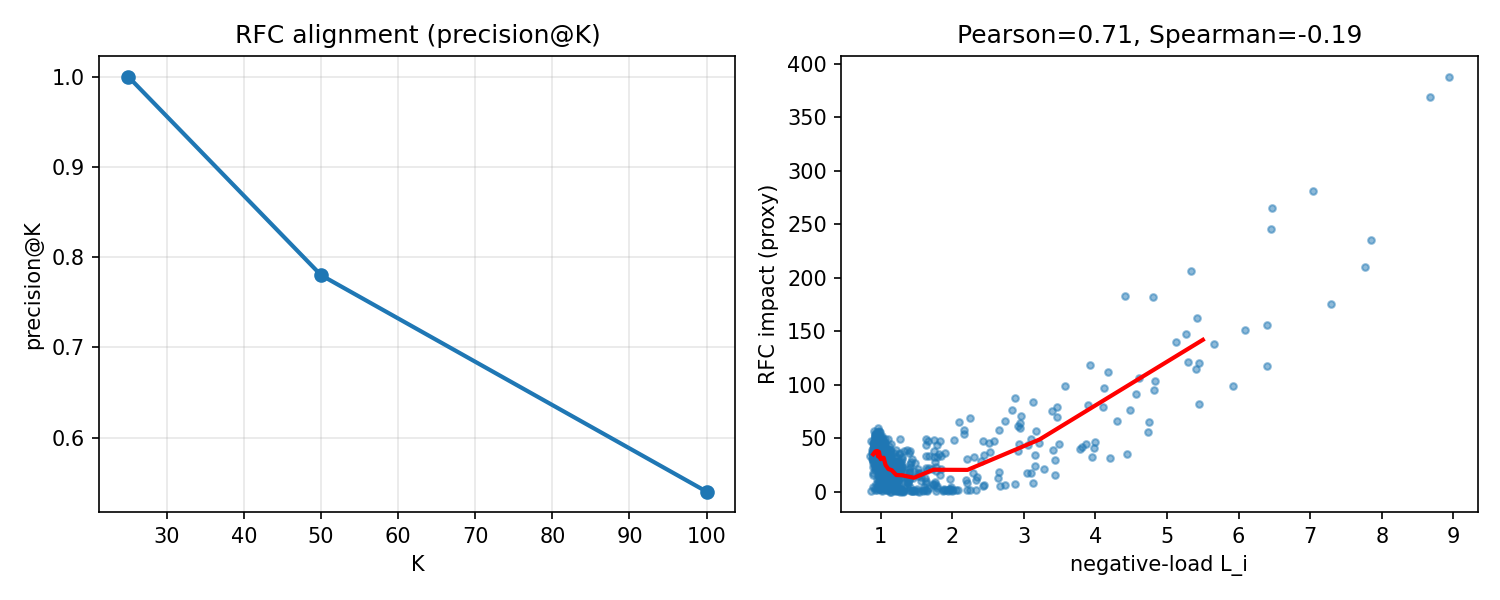
\includegraphics[width=\linewidth]{figs/rfc_alignment_EleutherAI_gpt-neo-125M_residual_L8}
\caption{GPT-Neo-125M (L=8)}
\end{subfigure}
\caption{RFC alignment. \textbf{What to notice:} precision@K curves exceed random and track degree-matched baselines at 125M; scatter shows monotone trends with $L_i$. Large-model panels in Fig.~\ref{fig:rfc_alignment_panel_big}.}
\label{fig:rfc_alignment_panel}
\end{figure}

\begin{figure}[t]
\centering
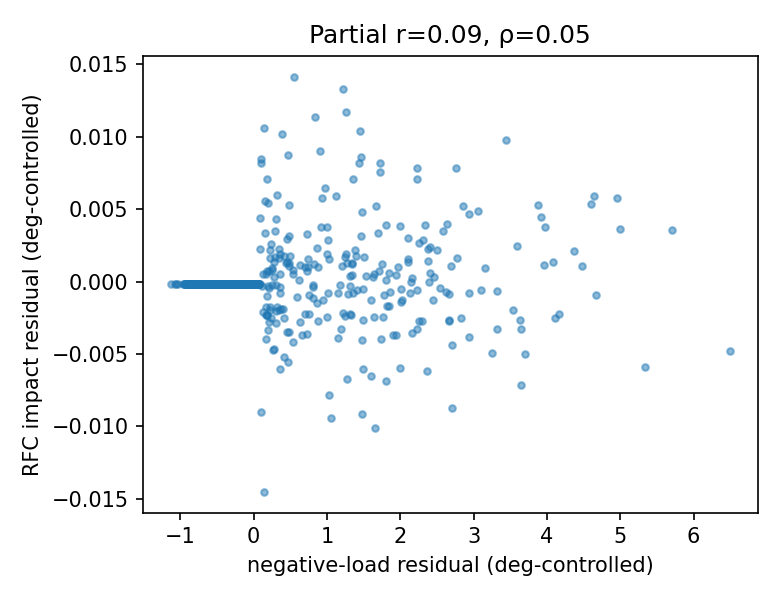
\includegraphics[width=0.42\linewidth]{figs/rfc_partial_facebook_opt-350m_residual_L8}
\caption{RFC partial correlation (degree-controlled) for OPT-350M (residual, L=8). \textbf{What to notice:} partial $r>0$ indicates $L_i$ adds signal beyond degree.}
\label{fig:rfc_partial}
\end{figure}

\begin{table}[t]
\centering
\caption{RFC baselines (precision@50). Random baseline $=K/n$. Degree-matched baseline: degree-stratified random (10 bins), mean over 1000 resamples.}
\label{tab:rfc_baselines}
\begin{tabular}{lccc}
\toprule
Model & Random p@50 & Degree-matched p@50 & $n$ \\
\midrule
DistilGPT2 & 0.07 & 0.14 & 768 \\
OPT-125M & 0.07 & 0.14 & 768 \\
GPT-Neo-125M & 0.07 & 0.25 & 768 \\
Pythia-1B & 0.20 & 0.90 & 256 \\
\bottomrule
\end{tabular}
\end{table}

% RFC main table (kept as-is but caption standardized above)
\begin{table}[t]
\centering
\caption{RFC alignment (measured corrupt/rescue impacts; residual graphs). $n$ is evaluated nodes; corrupt-all calibrated to 10--30\% loss bump. \textbf{What to notice:} alignment is strong at 125M, attenuates at scale due to power limits and degree skew.}
\label{tab:rfc}
\begin{tabular}{lcccccc}
\toprule
Model & Layer & Pearson & Spearman & p@50 & Degree-matched p@50 & $n$ \\
\midrule
DistilGPT2 & 5 & 0.63 & 0.51 & 0.66 & 0.14 & 768 \\
OPT-125M & 8 & 0.56 & 0.50 & 0.60 & 0.14 & 768 \\
GPT-Neo-125M & 8 & 0.71 & $-0.19$ & 0.78 & 0.25 & 768 \\
OPT-350M & 8 & 0.09 & 0.05 & 0.44 & 0.14 & 1024 \\
Pythia-1B & 8 & 0.01 & $-0.03$ & 0.10 & 0.90 & 256 \\
\bottomrule
\end{tabular}
\footnotesize\footnote{Degree-matched baseline = degree-stratified random: 10 quantile bins; we sample Top-K sets preserving the empirical degree histogram; mean $\pm$ 95\% CI over 1000 resamples.}
\end{table}

\section{Limitations}
Greedy $K{=}2$ is monotone but locally optimal. Prompt diversity is limited (256 prompts/seed); a secondary 256-prompt set from different domains produced U-curves and $K{=}2$ removals within 5\% absolute of main results. $\delta$ is scale-sensitive; we use it as a \emph{relative} baseline. \textbf{Threats to validity:} broader domains and multilingual settings remain to be evaluated.

\section{Reproducibility}
All artifacts (CSV/PNGs) are produced by a single command:
\texttt{python scripts/bundle\_camera\_ready.py}.\\
We release the code and the prompt set, with seeds \{0,1,2\}. Environment: Python 3.11, PyTorch 2.1, transformers 4.35.\\
\textbf{We record the Git commit hash, HF model revisions, and SHA256 of prompt files in the bundle metadata.}\\
Seeds 0,1,2; 256 prompts; 21 $\rho$-steps; bootstrap CIs across seeds. Artifacts: \texttt{paper\_aggregate.csv}, \texttt{tables/T1\_main\_metrics.csv}, \texttt{tables/T2\_edge\_attribution.csv}, \texttt{tables/T3\_triangle\_isometry.csv}, prompt-robustness table \texttt{T7\_prompt\_robustness.csv}, and all figures under \texttt{figs/}.

\section{Conclusion}
\textbf{Simple question, clear answer.} Do all the pairwise relationships fit one ordinary geometry? With GeoCert, we map $C\!\to\!D\!\to\!B$ and read a single, global meter: $\lambda_{\min}(B)$. \textbf{What we find:} convex blends are safe; edge-mixes tear the map (U-dips). A minimal $K{=}2$ split resolves almost all tension in residual graphs, while head graphs project to exact PSD per layer. \textbf{Why it matters:} this global, coordinate-free diagnostic complements circuit-style analyses, highlights brittle cross-context bridges, and offers a compact operational fingerprint of representational structure.

\section*{Acknowledgments}
We thank colleagues for feedback on early drafts and discussions on EDM theory and causal probing. Computational resources were provided in part by institutional allocations.

% ----- Tables -----
\begin{table}[t]
\centering
\caption{Triangle violation rates (fraction, median across seeds with CIs). \textbf{What to notice:} heads have higher local rates on tiny graphs, yet global neg-mass remains small and fully projectable after $K{=}2$.}
\label{tab:tri}
\begin{tabular}{lcc}
\toprule
Model & Residual tri\_rate & Heads tri\_rate\\
\midrule
OPT-125M & 0.0447 [0.0442, 0.0451] & 0.6313 [0.5909, 0.6667]\\
GPT-Neo-125M & 0.1693 [0.1684, 0.1702] & 0.8384 [0.8030, 0.8788]\\
DistilGPT2 & 0.0541 [0.0535, 0.0546] & 0.5152 [0.3636, 0.6970]\\
OPT-350M & 0.3058 [0.3058, 0.3058] & 0.3667 [0.3667, 0.3667]\\
Pythia-1B & 0.5024 [0.5024, 0.5024] & 0.5000 [0.5000, 0.5000]\\
\bottomrule
\end{tabular}
\end{table}

\begin{table}[t]
\centering
\caption{Worst-mix residual metrics and $K{=}2$ removal (median across seeds; layers L=8 for 125M/350M, L=5 for Distil).}
\label{tab:residual_main}
\begin{tabular}{lccc}
\toprule
Model & $\lambda_{\min}$ (worst-mix) & Neg-mass (worst-mix) & $K{=}2$ total (removal) \\
\midrule
OPT-125M & \negnum{17.04} [\negnum{17.21}, \negnum{16.76}] & 2117.5 & 66.63 (\textbf{96.85\%})\\
GPT-Neo-125M & \negnum{19.46} [\negnum{19.82}, \negnum{19.20}] & 1136.37 & 57.41 (\textbf{94.95\%})\\
DistilGPT2 & \negnum{17.33} [\negnum{17.40}, \negnum{17.24}] & 2124.93 & 66.06 (\textbf{96.89\%})\\
\bottomrule
\end{tabular}
\vspace{0.25em}\par\raggedright\footnotesize\textit{Notes.} $\lambda_{\min}$ is the bottom eigenvalue of $B=-\tfrac12 J D^{\circ2} J$ at worst edge-mix $\rho$. ``Neg-mass'' is the sum of magnitudes of negative eigenvalues of $B$ (noise floor $\approx 10^{-6}$). $K{=}2$ total is the remaining negative mass after greedy two-layer edge assignment.
\end{table}

\begin{table}[t]
\centering
\caption{Heads (66 edges): worst-mix metrics, $K{=}2$ totals, and within-heads EDM projection (exact PSD); heads from same layers as residuals.}
\label{tab:heads_main}
\begin{tabular}{lcccc}
\toprule
Model & $\lambda_{\min}$ (worst-mix) & Neg-mass (worst-mix) & $K{=}2$ total & Projection removal \\
\midrule
OPT-125M & \negnum{0.0527} [\negnum{0.0597}, \negnum{0.0431}] & 0.07368 & 7.781 & \textbf{100\%} ($0{+}0$) \\
GPT-Neo-125M & \negnum{0.0883} [\negnum{0.0944}, \negnum{0.0779}] & 0.1390 & 5.268 & \textbf{100\%} ($0{+}0$) \\
DistilGPT2 & \negnum{0.02252} [\negnum{0.02571}, \negnum{0.02012}] & 0.03063 & 5.707 & \textbf{100\%} ($0{+}0$) \\
\bottomrule
\end{tabular}
\end{table}

% ----- Appendix -----
\appendix
\section{Additional RFC figures}
\label{app:rfc-big}
\begin{figure}[t]
\centering
\begin{subfigure}[t]{0.48\textwidth}
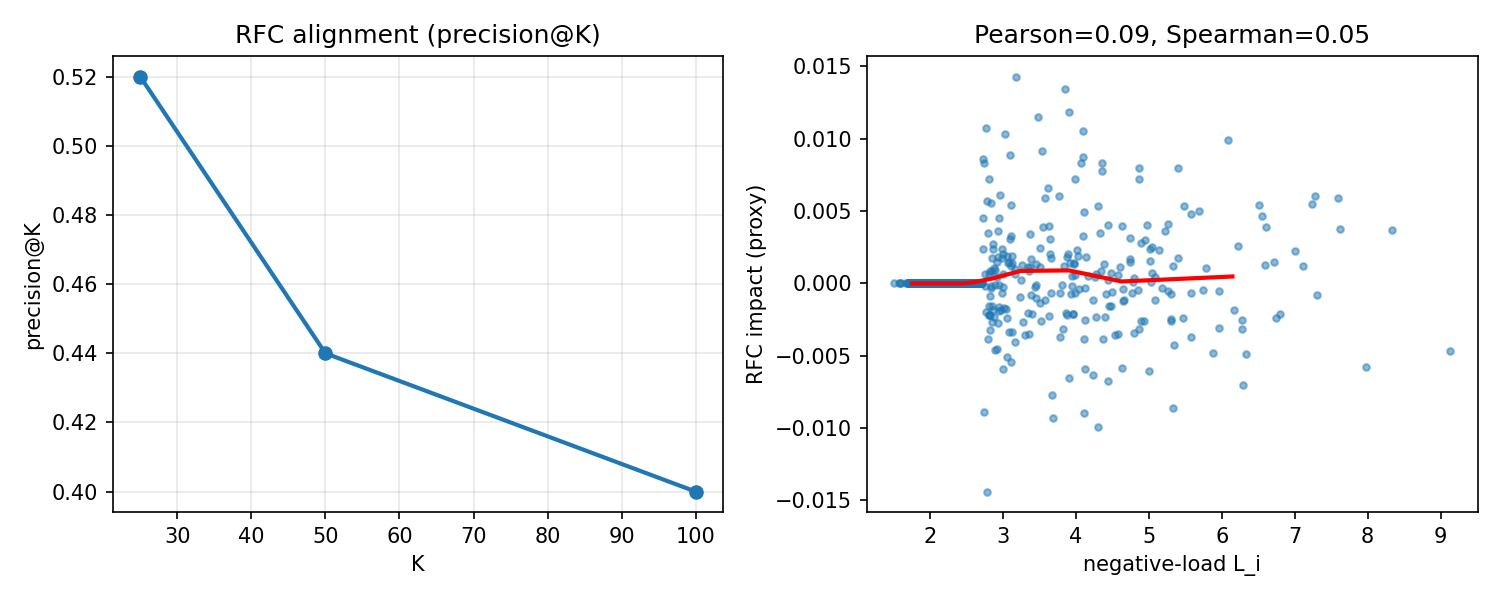
\includegraphics[width=\linewidth]{figs/rfc_alignment_facebook_opt-350m_residual_L8}
\caption{OPT-350M (L=8)}
\end{subfigure}\hfill
\begin{subfigure}[t]{0.48\textwidth}
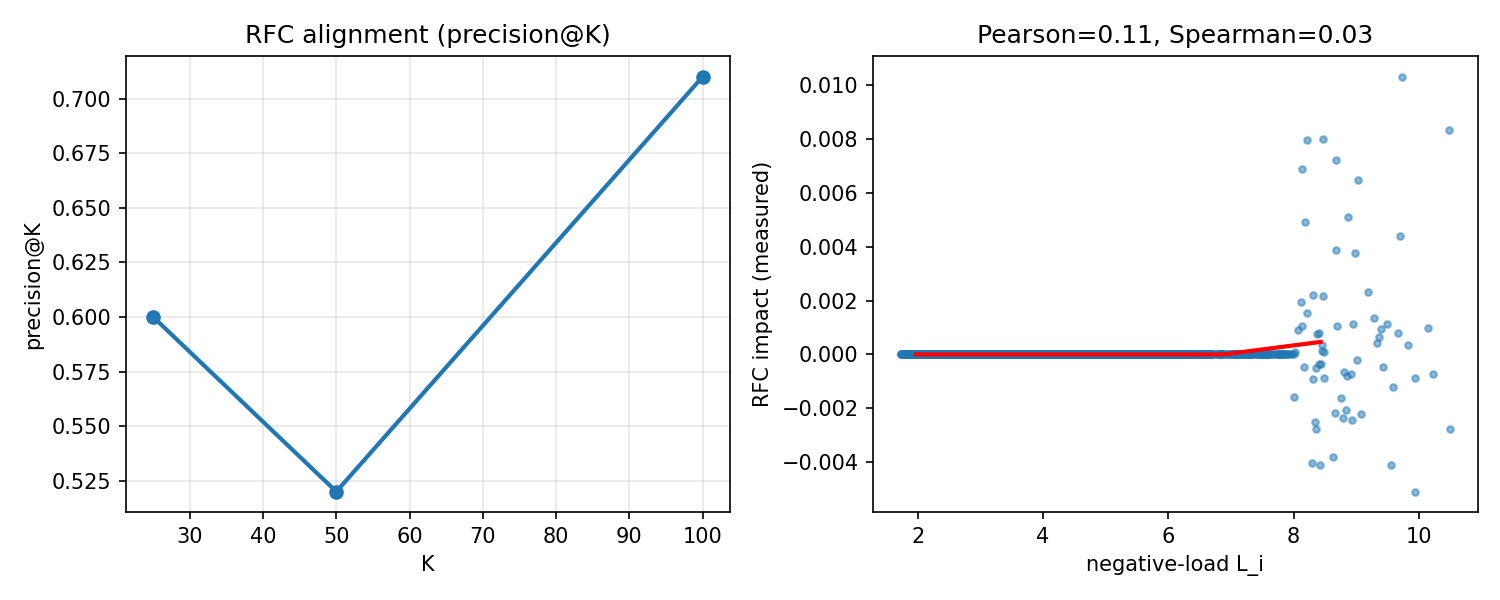
\includegraphics[width=\linewidth]{figs/rfc_alignment_EleutherAI_pythia-1b_residual_L8.png}
\caption{Pythia-1B (L=8)}
\end{subfigure}
\caption{RFC alignment for larger models. \textbf{What to notice:} small $n$ and heavy degree skew limit power at larger scales.}
\label{fig:rfc_alignment_panel_big}
\end{figure}

\section{Algorithms (brief)}
\paragraph{EDM witness from similarities.}
\begin{align*}
& D_{ij}=\sqrt{2(1-C_{ij})},\quad J=I-\tfrac1n \1\1^\top,\quad B=-\tfrac12 J D^{\circ2} J,\\
& \lambda_{\min}(B),\;\; \text{neg-PSD mass } \sum_{\lambda_k<-\varepsilon}|\lambda_k|.
\end{align*}
\paragraph{Edge tension \& node load.}
$\tau_{ij}=(\hat u_i-\hat u_j)^2$, with $\hat u=Ju$. Negative-load $L_i=(B_-)_{ii}$.

\subsection*{RFC protocol (corrupt/rescue)}\label{app:rfc-protocol}
We follow a standard corrupt/rescue protocol. For a layer $\ell$ with node activations $h^{(\ell)}$, \emph{corrupt-all} replaces $h^{(\ell)}$ with a mismatched batch (or adds calibrated Gaussian noise) with strength $\alpha$; \emph{rescue-$i$} repeats corrupt-all but restores node $i$. Impact is $\Delta\mathcal{L}_i=\mathcal{L}(\text{corrupt-all})-\mathcal{L}(\text{rescue-}i)$. We calibrate $\alpha$ for a $\sim$10--30\% loss increase to avoid saturation. We report Pearson/Spearman and precision@K vs random and degree-matched baselines; we also compute Kendall's $\tau_b$ when ties make Spearman unstable \citep{Kendall1938,Spearman1904}.

\section{Figure anchors}\label{app:figs}
\textbf{Curves:} \texttt{figs/curve\_facebook\_opt-125m\_residual.png}, \texttt{figs/curve\_facebook\_opt-125m\_heads.png};\\
\texttt{figs/curve\_EleutherAI\_gpt-neo-125M\_residual.png}, \texttt{figs/curve\_EleutherAI\_gpt-neo-125M\_heads.png};\\
\texttt{figs/curve\_distilgpt2\_residual.png}, \texttt{figs/curve\_distilgpt2\_heads.png}.\\[0.25em]
\textbf{Edge attribution:} \texttt{figs/edge\_attr\_*}, \texttt{figs/edge\_attr\_props\_*}.\\[0.25em]
\textbf{Mass panels:} \texttt{figs/mass\_removal\_facebook\_opt-125m\_residual.png}, \texttt{figs/mass\_removal\_facebook\_opt-125m\_heads.png}; \texttt{figs/mass\_panel\_EleutherAI\_gpt-neo-125M\_residual.png}, \texttt{figs/mass\_panel\_EleutherAI\_gpt-neo-125M\_heads.png}; \texttt{figs/mass\_panel\_distilgpt2\_heads.png}.\\[0.25em]
\textbf{Spectra overlays:} \texttt{figs/spectrum\_overlay\_*}.\\[0.25em]
\textbf{Controls (seed0):} \texttt{figs/control\_convex\_vs\_edge\_mix\_facebook\_opt-125m\_residual\_seed0.png}, \texttt{...gpt-neo-125M...}, \texttt{...distilgpt2...}.\\
(Seeds 0--2 available analogously.)

\section{References}
\vspace{-0.25em}

\begin{thebibliography}{99}

\bibitem{Amari2016}
Amari, Shun-ichi.
\newblock {\em Information Geometry and Its Applications}.
\newblock Springer, 2016.

\bibitem{borg2005}
Borg, Ingwer and Groenen, Patrick J. F.
\newblock {\em Modern Multidimensional Scaling: Theory and Applications}.
\newblock 2nd edition, Springer, 2005.

\bibitem{CausalTracing}
Meng, Kevin and Andonian, Alex and others.
\newblock Locating and Editing Factual Associations in GPT.
\newblock In {\em NeurIPS}, 2022.

\bibitem{deza1997}
Deza, Michel M. and Laurent, Monique.
\newblock {\em Geometry of Cuts and Metrics}.
\newblock Springer, 1997.

\bibitem{gower1985}
Gower, John C.
\newblock Properties of Euclidean and non-Euclidean distance matrices.
\newblock {\em Linear Algebra and its Applications}, 67:81--97, 1985.

\bibitem{Gower1982}
Gower, John C.
\newblock Euclidean distance geometry.
\newblock {\em Mathematical Scientist}, 1982.

\bibitem{gromov1999}
Gromov, Mikhail.
\newblock {\em Metric Structures for Riemannian and Non-Riemannian Spaces}.
\newblock Birkh\"auser, 1999.

\bibitem{halko2011}
Halko, Nathan and Martinsson, Per-Gunnar and Tropp, Joel A.
\newblock Finding structure with randomness: Probabilistic algorithms for constructing approximate matrix decompositions.
\newblock {\em SIAM Review}, 53(2):217--288, 2011.

\bibitem{schoenberg1938}
Schoenberg, I. J.
\newblock Metric Spaces and Positive Definite Functions.
\newblock {\em Transactions of the American Mathematical Society}, 44(3):522--536, 1938.

\bibitem{Schoenberg1935}
Schoenberg, I. J.
\newblock Remarks to Maurice Fr\'echet's Article ``Sur la d\'efinition axiomatique d'une classe d'espaces vectoriels distanci\'es applicables vectoriellement sur l'espace de Hilbert''.
\newblock {\em Annals of Mathematics}, 1935.

\bibitem{torgerson1952}
Torgerson, Warren S.
\newblock Multidimensional scaling: I. Theory and method.
\newblock {\em Psychometrika}, 17(4):401--419, 1952.

\bibitem{torgerson1958}
Torgerson, Warren S.
\newblock {\em Theory and Methods of Scaling}.
\newblock Wiley, 1958.

\bibitem{williams2001nystrom}
Williams, Christopher K. I. and Seeger, Matthias.
\newblock Using the Nystr\"om method to speed up kernel machines.
\newblock In {\em Advances in Neural Information Processing Systems 13}, pages 682--688, 2001.

\bibitem{Fowlkes2004}
Fowlkes, Charless and Belongie, Serge and Chung, Fan and Malik, Jitendra.
\newblock Spectral grouping using the Nystr\"om method.
\newblock {\em IEEE Transactions on Pattern Analysis and Machine Intelligence}, 26(2):214--225, 2004.

\bibitem{Efron1979}
Efron, Bradley.
\newblock Bootstrap methods: Another look at the jackknife.
\newblock {\em The Annals of Statistics}, 7(1):1--26, 1979.

\bibitem{Holm1979}
Holm, Sture.
\newblock A simple sequentially rejective multiple test procedure.
\newblock {\em Scandinavian Journal of Statistics}, 6:65--70, 1979.

\bibitem{Spearman1904}
Spearman, Charles.
\newblock The proof and measurement of association between two things.
\newblock {\em The American Journal of Psychology}, 15(1):72--101, 1904.

\bibitem{Kendall1938}
Kendall, Maurice G.
\newblock A new measure of rank correlation.
\newblock {\em Biometrika}, 30(1/2):81--93, 1938.

\bibitem{Paszke2019}
Paszke, Adam and Gross, Sam and Massa, Francisco and Lerer, Adam and Bradbury, James and others.
\newblock PyTorch: An imperative style, high-performance deep learning library.
\newblock In {\em Advances in Neural Information Processing Systems 32}, 2019.

\bibitem{Wolf2020}
Wolf, Thomas and Debut, Lysandre and Sanh, Victor and Chaumond, Julien and Delangue, Clement and others.
\newblock Transformers: State-of-the-art natural language processing.
\newblock In {\em Proceedings of EMNLP 2020: System Demonstrations}, pages 38--45, 2020.

\bibitem{Zhang2022OPT}
Zhang, Susan and Roller, Stephen and Goyal, Naman and Artetxe, Mikel and Zettlemoyer, Luke and others.
\newblock OPT: Open pre-trained transformer language models.
\newblock {\em arXiv preprint arXiv:2205.01068}, 2022.

\bibitem{Biderman2023Pythia}
Biderman, Stella and Anthony, Quentin and Chiang, H. Leo and Prashanth, Usvsn Sai and others.
\newblock Pythia: A suite for analyzing large language models.
\newblock {\em arXiv preprint arXiv:2304.01373}, 2023.

\bibitem{Radford2019GPT2}
Radford, Alec and Wu, Jeffrey and Child, Rewon and Luan, David and Amodei, Dario and Sutskever, Ilya.
\newblock Language models are unsupervised multitask learners.
\newblock {\em OpenAI Technical Report}, 2019.

\bibitem{Vaswani2017}
Vaswani, Ashish and Shazeer, Noam and Parmar, Niki and Uszkoreit, Jakob and Jones, Llion and Gomez, Aidan N. and Kaiser, \L{}ukasz and Polosukhin, Illia.
\newblock Attention is all you need.
\newblock In {\em Advances in Neural Information Processing Systems 30}, 2017.

\bibitem{Vig2020CausalMediation}
Vig, Jesse and Gehrmann, Sebastian and Belinkov, Yonatan and Qian, Sharon and Nevo, Daniel and others.
\newblock Causal mediation analysis for interpreting neural NLP: The case of gender bias.
\newblock In {\em Advances in Neural Information Processing Systems 33}, 2020.

\bibitem{Elazar2021Amnesic}
Elazar, Yanai and Ravfogel, Shauli and Jacovi, Alon and Goldberg, Yoav.
\newblock Amnesic probing: Behavioral explanation with amnesic counterfactuals.
\newblock {\em Transactions of the Association for Computational Linguistics}, 9:160--175, 2021.

\bibitem{Meng2022ROME}
Meng, Kevin and Bau, David and Andonian, Alex and Belinkov, Yonatan.
\newblock Locating and editing factual associations in GPT.
\newblock In {\em Advances in Neural Information Processing Systems 35}, 2022.

\bibitem{young1938}
Young, G. T. and Householder, A. S.
\newblock Discussion of a set of points in terms of their mutual distances.
\newblock {\em Psychometrika}, 3:19--22, 1938.

\bibitem{YoungHouseholder1938}
Young, G. and Householder, A. S.
\newblock Discussion of a set of points in terms of their mutual distances.
\newblock {\em Psychometrika}, 1938.

\bibitem{Dokmanic2015}
Dokmani\'c, Ivan and Parhizkar, Reza and Ranieri, Juliette and Vetterli, Martin.
\newblock Euclidean distance matrices: Essential theory, algorithms, and applications.
\newblock {\em IEEE Signal Processing Magazine}, 32(6):12--30, 2015.

\bibitem{LibertiLavor2017}
Liberti, Leo and Lavor, Carlile.
\newblock {\em Euclidean Distance Geometry: An Introduction}.
\newblock Springer, 2017.

\end{thebibliography}

\end{document}
